%===========================================================
%
% Dedman/Lyle LaTeX Dissertation Template, v.2016
% Structure organized by Ted C. Munger (TCM)
%
%===========================================================
%===========================================================
% BEGIN Document Style
%===========================================================
\documentclass[12pt, final]{scrreprt}

\makeatletter
\DeclareOldFontCommand{\rm}{\normalfont\rmfamily}{\mathrm}
\DeclareOldFontCommand{\sf}{\normalfont\sffamily}{\mathsf}
\DeclareOldFontCommand{\tt}{\normalfont\ttfamily}{\mathtt}
\DeclareOldFontCommand{\bf}{\normalfont\bfseries}{\mathbf}
\DeclareOldFontCommand{\it}{\normalfont\itshape}{\mathit}
\DeclareOldFontCommand{\sl}{\normalfont\slshape}{\@nomath\sl}
\DeclareOldFontCommand{\sc}{\normalfont\scshape}{\@nomath\sc}
\makeatother


  \usepackage{DL_thesis_v2016}  % TCM Global Style for particular SMU College, e.g. DL_thesis_v2016.sty

  %--------------------------------------------------------------------------------------------------------
% 									LaTeX Package File
%
% TCM Use this file to add, modify, or comment out packages you want to utilize in your Latex project.
%     This file must be included in the main document file.
%--------------------------------------------------------------------------------------------------------

\usepackage{adjustbox}       % TCM Extends the graphicx package to do trimming and other adjustments.
\usepackage{algorithm}       % TCM Algorithm block See http://algorithms.berlios.de/
\usepackage{algorithmic}     % TCM Algorithm & Peudocode See http://en.wikibooks.org/wiki/LaTeX/Algorithms_and_Pseudocode
\usepackage{amsmath}         % Need for subequations
%\usepackage{amssymb}        % amssymb-telda and math symbols
\usepackage{booktabs}        % TCM Allows fancy Tables
\usepackage{boxedminipage}   % Boxes around figures
\usepackage{breqn}           % TCM Automatically breaks long equation lines - usually
\usepackage{changepage} 	 % TCM Allows one to temporarily change right and left margins
\usepackage{cite} 	 		 % TCM Allows improved handling of numeric citations including automatic ordering and ranges of multiple cites
\usepackage{enumitem} 		 % TCM Allows one to easily change the labels for enumerate list
%\usepackage{epsf}           % TCM This EPS file package is greatly depreciated for the graphicx package bundle. Use at own risk.
\usepackage{fancyhdr}
\usepackage{flafter}         % Floats should always appear after their definition
\usepackage[flushleft]{threeparttable}  % TCM This package allows for notes under tables.  Flushleft option flushes the note left margin of table (center is default)
\usepackage{geometry}		 % TCM Allows to customize paper size and margins.
\usepackage{graphicx}        % TCM Extends graphics package for figures. Provides op­tional ar­gu­ments to the \in­clude­graph­ics com­mand
\usepackage{epstopdf}        % TCM Converts eps images to PDF to use in graphicx package.  Must be loaded after graphicx package
\usepackage{longtable}       % TCM Allows for Automatic page breaks for long tables
%\usepackage{jneurosci}       % TCM The jneurosci bibliography style makes use of some commands - for example, \citeauthoryear.  Must include if using named or acmsmall bib style
\usepackage{ltablex}		 % TCM Modifies Tabularx Package by combining properties of tabularx and longtable.
\usepackage[maxfloats=36]{morefloats}      % Latex will handle more floats 18-36
\usepackage{moresize}        % TCM Adds \HUGE and \ssmall font sizes
\usepackage{multirow}        % TCM Allows multirow cells in tables (similar to merge and center in Excel)
%\usepackage{named}           % TCM Bibliography style that allows for more fine-tuned citing. Commands include \cite, \citeauthor, \citeyear and \shortcite (for after you've already used \citeauthor).
\usepackage{outlines}		 % TCM Needed for outlines
\usepackage{rotate}			 % TCM Performs rotations of floating environments (images w/ cations, etc)
\usepackage{rotating}        % Need for sidewaystable
\usepackage{scrextend}		 % TCM package that allows for KOMA-Script classes available for other classes: e.g., labeling lists etc.  See package documentation for further information.
\usepackage{pdflscape}		 % TCM Allows Landscape Page
%%\usepackage{qtree}         % Need for trees
\usepackage{setspace}        % TCM Allows for more intuitive commands for single and double spacing
\usepackage{siunitx}		 % TCM package required to ensure units are typeset properly with numbers e.g. \SI{10}{\kg\m\per\square\s}
\sisetup{output-exponent-marker=\ensuremath{\mathrm{E}}}  % TCM Option allows for Scientific notation of Numbers.  Format is \num{#.####E##}
% \usepackage[superscript]{cite}		  % TCM Makes citations superscript instead of [#]
\usepackage [table]{xcolor}	 % TCM Allows coloring of tables
\usepackage{tabularx}		 % TCM Package which allows paragraphs in Tables
% \usepackage{thumbpdf}		  % TCM Comment out as causes warnings, can easily create thumbs in Adobe if needed.

%===========================================================
% BEGIN Color ToDo Comment Notes for editing
%===========================================================
\usepackage[colorinlistoftodos,textwidth=25mm,shadow,backgroundcolor=green]{todonotes}				  % TCM Allows margin comments
\usepackage{marginnote}				  % TCM Require for Todonotes in Align Envionment
  %~~~~~~~~~~~~~~~~~~~~~~~~~~~~~~~~~~~~~~~~~~~~~~~~~~~~~~~~~~~
  % TCM  BEGIN Altering Todonotes Commands to use Marginnote instead of Marginpar to use todonotes in align environment
%~~~~~~~~~~~~~~~~~~~~~~~~~~~~~~~~~~~~~~~~~~~~~~~~~~~~~~~~~~~
     \makeatletter
     \renewcommand{\@todonotes@drawMarginNoteWithLine}{%
     \begin{tikzpicture}[remember picture, overlay, baseline=-0.75ex]%
         \node [coordinate] (inText) {};%
     \end{tikzpicture}%
     \marginnote[{% Draw note in left margin
         \@todonotes@drawMarginNote%
      \@todonotes@drawLineToLeftMargin%
     }]{% Draw note in right margin
         \@todonotes@drawMarginNote%
         \@todonotes@drawLineToRightMargin%
     }%
     }
     \makeatother
       %----------------------------------------------------
       % TCM  BEGIN New Todonotes Command to use single line spacing (sls) in note
       %----------------------------------------------------
       \newcommand{\slstodo}[2][]
       {\todo[caption={#2}, size=\small, #1]{\renewcommand{\baselinestretch}{0.5}\selectfont#2\par}}
       %----------------------------------------------------
       % TCM  END New Todonotes Command to use single spacing in note
       %----------------------------------------------------
       
  %~~~~~~~~~~~~~~~~~~~~~~~~~~~~~~~~~~~~~~~~~~~~~~~~~~~~~~~~~~~
  % TCM  END Altering Todonotes Commands to use Marginnote instead of Marginpar to use todonotes in align 
%~~~~~~~~~~~~~~~~~~~~~~~~~~~~~~~~~~~~~~~~~~~~~~~~~~~~~~~~~~~
%===========================================================
% END Color ToDo Comment Notes for editing
%===========================================================

\usepackage{verbatim}        % TCM Verbatim text block
\usepackage{wrapfig}         % Wrap figures
\usepackage{xspace}          % Allows dynamic space in global text variables. This can allow you to just use \newCommandName rather than \newCommandName{}.
\usepackage [bookmarks=true,backref=page, hyperfigures=true, pdfpagelabels=false] {hyperref}
%===========================================================
% BEGIN Hyperlink Setup
%===========================================================
\hypersetup{
									  % TCM Added more precise definition and options for Hyperref package.
									  % TCM Comment out or change hyperref preferences
									  % TCM \hypersetup should be loaded last 
    bookmarksopen=true,				  % True: Open bookmark tree
    bookmarksnumbered=true, 		  % True: put section numbers in bookmarks
    breaklinks=true,				  % True: split the url over multiple lines
%    draft=true,						  % True: do not do any hyper linking
    filecolor=magenta, 				  % Color of file links
    citecolor=blue, 				  % Color of links to bibliography
    colorlinks=true, 				  % False: boxed links; true: colored links
    linkcolor=blue, 				  % Color of internal links
    linktocpage=true, 				  % True: Makes the page number of TOC the link vs the text
%    pagebackref=true,				  % True: Links references back to referring page
    pdfnewwindow=true,         		  % True: URL links in new window
    plainpages=false, 				  % True: do page number anchors as plain Arabic
    pdffitwindow=false,        		  % Window fit to page when opened
    pdfmenubar=true,           		  % Show Acrobat menu
    pdfstartview={FitH},       		  % Fits the width of the page to the window
    pdftoolbar=true, 				  % Show Acrobat toolbar
    pdfauthor={Author}, 			  % Author in PDF document properties
    pdfcreator={Author}, 			  % Creator of the document in PDF document properties
    pdfkeywords={Keyword1} {Keyword2} {Keyword3} {Keyword4} {Author}, % List of keywords in PDF document properties
    pdfproducer={Producer}, 		  % Producer of the document in PDF document properties
    pdfsubject={Subject},   % Subject of the document in PDF document properties
    pdftitle={Title of Dissertation}, % Title in PDF document properties
    unicode=false,             		  % Non-Latin characters in Acrobat bookmarks
    urlcolor=cyan 					  % Color of external links
}
%===========================================================
% END Hyperlink Setup
%===========================================================
\usepackage{bookmark}		 		  % TCM Eliminates Warning Bookmark level greater than one.  Must be loaded after Hyperref

%===========================================================
% Arya's Packages
%===========================================================
\usepackage{tgpagella}		 		  % ADM Let's use Papyrus. It really classes up this whole affair.
\usepackage{microtype}		 		  % ADM While we're at it, so does improved kerning.
% \usepackage[font=small,labelfont=bf,hypcap]{caption}
%\usepackage{mathtools, amsmath, amsfonts, amssymb}
\usepackage{dirtytalk}
\usepackage{bm}  % ADM Bold math symbols
               % Packages File

  \geometry{letterpaper, margin=1in} % TCM Dedman/Lyle Standard 2016


  \linespread{1.6}
  \setcounter{secnumdepth}{4} % TCM Sets number subsections
  \setcounter{tocdepth}{4}    % TCM Set the number of subsections in TOC
  
   \urlstyle{same} % TCM Set URL style to same font as text verses mono-spaced, i.e., courier

%===========================================================
% END Document Style
%===========================================================
%===========================================================
% BEGIN Insert Custom Commands
%===========================================================
  %======================================================================
% Custom Commands  Inital Creation TCM 2015
%======================================================================
% Use this document to place all of your global new commands
%======================================================================

%======================================================================
% BEGIN SMU Custom Commands
%======================================================================
% The many of the following commands were originally in the smu_thesis.sty
% file. Commands and comments were moved here to make style file more about
% document style. While custom environments can technically be considered 
% style, the student created environments are included here to simplify
% the style file. Often these commands were created by students over the
% years and placed in the style file.  The commands have not been 
% verified and can be obsolete LaTeX commands. The Commands can be used 
% or ignored. 
%======================================================================
%----------------------------------------------------------------------
% BEGIN TCM Commands to set formatting for Paragraph section to have line
%           feed after heading & Numbered. This custom command makes
%           \paragraph, in essence, a form of \subsubsubsection.
%           Uncomment to use.
%----------------------------------------------------------------------
%  \makeatletter
%  \renewcommand\paragraph{\@startsection{paragraph}{4}{\z@}%
%    {-3.25ex\@plus -1ex \@minus -.2ex}%
%    {1.5ex \@plus .2ex}%
%    {\normalfont\normalsize\bfseries}}
%  \makeatother
%----------------------------------------------------------------------
% END of Commands to set formatting for Paragraph section to have line
%       feed after heading TCM
%----------------------------------------------------------------------
%----------------------------------------------------------------------
% BEGIN Shortcuts to insert calligraphic letters in Math Mode Only
%----------------------------------------------------------------------
\newcommand{\cA}{{\mathcal A}}
\newcommand{\cB}{{\mathcal B}}
\newcommand{\cC}{{\mathcal C}}
\newcommand{\cD}{{\mathcal D}}
\newcommand{\cE}{{\mathcal E}}
\newcommand{\cF}{{\mathcal F}}
\newcommand{\cG}{{\mathcal G}}
\newcommand{\cH}{{\mathcal H}}
\newcommand{\cI}{{\mathcal I}}
\newcommand{\cJ}{{\mathcal J}}
\newcommand{\cK}{{\mathcal K}}
\newcommand{\cL}{{\mathcal L}}
\newcommand{\cM}{{\mathcal M}}
\newcommand{\cN}{{\mathcal N}}
\newcommand{\cO}{{\mathcal O}}
\newcommand{\cP}{{\mathcal P}}
\newcommand{\cQ}{{\mathcal Q}}
\newcommand{\cR}{{\mathcal R}}
\newcommand{\cS}{{\mathcal S}}
\newcommand{\cT}{{\mathcal T}}
\newcommand{\cU}{{\mathcal U}}
\newcommand{\cV}{{\mathcal V}}
\newcommand{\cW}{{\mathcal W}}
\newcommand{\cX}{{\mathcal X}}
\newcommand{\cY}{{\mathcal Y}}
\newcommand{\cZ}{{\mathcal Z}}
% Lower case caligraphy letters
\newcommand{\cw}{{\mathcal w}}
%----------------------------------------------------------------------
% END Shortcuts to insert calligraphic letters in Math Mode Only
%----------------------------------------------------------------------
%----------------------------------------------------------------------
% BEGIN Shortcuts to insert boldface letters 
%----------------------------------------------------------------------
\newcommand{\bA}{{\bf A}}
\newcommand{\bB}{{\bf B}}
\newcommand{\bC}{{\bf C}}
\newcommand{\bD}{{\bf D}}
\newcommand{\bE}{{\bf E}}
\newcommand{\bF}{{\bf F}}
\newcommand{\bG}{{\bf G}}
\newcommand{\bH}{{\bf H}}
\newcommand{\bI}{{\bf I}}
\newcommand{\bJ}{{\bf J}}
\newcommand{\bK}{{\bf K}}
\newcommand{\bL}{{\bf L}}
\newcommand{\bM}{{\bf M}}
\newcommand{\bN}{{\bf N}}
\newcommand{\bO}{{\bf O}}
\newcommand{\bP}{{\bf P}}
\newcommand{\bQ}{{\bf Q}}
\newcommand{\bR}{{\bf R}}
\newcommand{\bS}{{\bf S}}
\newcommand{\bT}{{\bf T}}
\newcommand{\bU}{{\bf U}}
\newcommand{\bV}{{\bf V}}
\newcommand{\bW}{{\bf W}}
\newcommand{\bX}{{\bf X}}
\newcommand{\bY}{{\bf Y}}
\newcommand{\bZ}{{\bf Z}}
%----------------------------------------------------------------------
% END Shortcuts to insert boldface letters 
%----------------------------------------------------------------------
%----------------------------------------------------------------------
% BEGIN Shortcuts to insert overline symbols in Math Mode Only
%----------------------------------------------------------------------
\newcommand{\oA}{{\overline A}}
\newcommand{\oB}{{\overline B}}
\newcommand{\oC}{{\overline C}}
\newcommand{\oD}{{\overline D}}
\newcommand{\oE}{{\overline E}}
\newcommand{\oF}{{\overline F}}
\newcommand{\oG}{{\overline G}}
\newcommand{\oH}{{\overline H}}
\newcommand{\oI}{{\overline I}}
\newcommand{\oJ}{{\overline J}}
\newcommand{\oK}{{\overline K}}
\newcommand{\oL}{{\overline L}}
\newcommand{\oM}{{\overline M}}
\newcommand{\oN}{{\overline N}}
\newcommand{\oO}{{\overline O}}
\newcommand{\oP}{{\overline P}}
\newcommand{\oQ}{{\overline Q}}
\newcommand{\oR}{{\overline R}}
\newcommand{\oS}{{\overline S}}
\newcommand{\oT}{{\overline T}}
\newcommand{\oU}{{\overline U}}
\newcommand{\oV}{{\overline V}}
\newcommand{\oW}{{\overline W}}
\newcommand{\oX}{{\overline X}}
\newcommand{\oY}{{\overline Y}}
\newcommand{\oZ}{{\overline Z}}
% Lower case overline
\newcommand{\ovd}{{\overline d}}
\newcommand{\ove}{{\overline e}}
\newcommand{\ovf}{{\overline f}}
\newcommand{\ovg}{{\overline g}}
\newcommand{\ovh}{{\overline h}}
\newcommand{\ovi}{{\overline i}}
%----------------------------------------------------------------------
% END Shortcuts to insert overline symbols in Math Mode Only
%----------------------------------------------------------------------
%----------------------------------------------------------------------
% BEGIN Shortcuts to insert vector symbols in Math Mode Only
%----------------------------------------------------------------------
\newcommand{\vS}{{\vec S}}
\newcommand{\vT}{{\vec T}}
\newcommand{\vU}{{\vec U}}
\newcommand{\vV}{{\vec V}}
\newcommand{\vW}{{\vec W}}
\newcommand{\vX}{{\vec X}}
\newcommand{\vY}{{\vec Y}}
\newcommand{\vZ}{{\vec Z}}
% Lower case vectors
\newcommand{\vs}{{\vec s}}
\newcommand{\vt}{{\vec t}}
\newcommand{\vu}{{\vec u}}
\newcommand{\vv}{{\vec v}}
\newcommand{\vw}{{\vec w}}
\newcommand{\vx}{{\vec x}}
%----------------------------------------------------------------------
% END Shortcuts to insert vector symbols in Math Mode Only
%----------------------------------------------------------------------
%----------------------------------------------------------------------
% BEGIN Misc. Commands defined by students
%----------------------------------------------------------------------
\newcommand{\myqed}{\vspace{-1.1cm} \qed \vspace{0.9cm}}
\newcommand{\qed}{\mbox{$\ \Box$}}
\newcommand{\lqed}{\qed\vspace{.1in}}
\newcommand{\nf}{{\mbox{$\sim$}}}
\newcommand{\wt}{\mbox{$\widehat{T}$}}
\newcommand{\as}{\mbox{$/\hspace{-2mm}>$}}
\newcommand{\equi}{\mbox{$\leftrightarrow$}}
\newcommand{\myeq}{\mbox{$\leftrightarrow$}}
%\newcommand{\tab}{\hspace*{4em}}
%\newcommand{\ind}{\hspace*{2em}}
%\newcommand{\mif}{\mbox{ :- }}
%\newcommand{\dd}{\mbox{$\bullet$}}
\newcommand{\dd}{\mbox{\ $\mid$\ }}

\newcommand{\ind}{\hspace*{2.0em}}
\newcommand{\tab}{\hspace*{4em}}

\newcommand{\myp}{\protect{$+$}}
\newcommand{\mypp}[1]{\protect{${#1}$}}
\newcommand{\myf}[2]{\protect{\ \(\frac{\mbox{\rm #1}}{\mbox{\rm #2}}\)}\ }
\newcommand{\myup}{\protect{$ \uparrow$}}
\newcommand{\scc}[1]{\protect{\ \ \ $ SCC = {#1} $}}

% \newcommand{\twoheadrightarrow}{{\rightarrow \hspace{-0.3cm} \rightarrow \hspace{0.2cm}}}

\newcommand{\chap}[1]{\chapter{\protect{\bf {#1}}}}
\newcommand{\mytab}{\hspace*{13em}}
\newcommand{\bleft}{\left \{\ }
\newcommand{\bright}{\ \right \}}
\newcommand{\sind}{ \ \ \ }
\newcommand{\mand}{ \ \&\ }
\newcommand{\mif}{\mbox{\ :-\ }}
%%%\newcommand{\nf}{\sim}
\newcommand{\posI}{$I^+$}
\newcommand{\negI}{$I^-$}
%\newcommand{\AST}{$AST(P)$}
\newcommand{\Ip}[1]{${\mathcal I}_{#1}$}
\newcommand{\II}[1]{${\mathcal I}({#1})$}
%\newcommand{\HU}[1]{${\mathcal HU}_{#1}$}
%\newcommand{\US}{${\mathcal US}$}
%\newcommand{\HB}[1]{${\mathcal HB}_{#1}$}
%----- chen  -----------------
%\newcommand{\emptyset}{\phi}
\newcommand{\cUS}{{\mathcal US}}
\newcommand{\cHU}{{\mathcal HU}}
\newcommand{\cHB}{{\mathcal HB}}
\newcommand{\cUC}{{\mathcal UC}s}
\newcommand{\cBody}{{\mathcal B}ody}
\newcommand{\wA}{\widetilde{\rm A}}
\newcommand{\LF}{${\mathcal LF}$}
\newcommand{\DI}{DI^+ \cup DI^-}
\newcommand{\AI}{AI^+ \cup AI^-}
\newcommand{\Asp}{\tt asp}
\newcommand{\Aspt}[1]{${\tt asp}({#1})$}
\newcommand{\BP}[1]{${\mathcal BP}({#1})$}
\newcommand{\myarrow}{-\hspace*{-0.23cm}-\hspace*{-0.23cm}-\hspace*{-0.23cm}\longrightarrow}
\newcommand{\nedge}{\rightarrow\hspace*{-0.39cm}{\prime} \hspace*{0.29cm}}
\newcommand{\jmp}[1] {\hspace*{0.3in}{#1}\hspace*{0.3in}}
\newcommand{\Aro}[1]{\stackrel{#1}\longrightarrow}
\newcommand{\MyAro}[1]{\stackrel{#1}\myarrow}
\newcommand{\MyLoAro}[1]{\stackrel{#1}{-\hspace*{-0.23cm}-\hspace*{-0.23cm}\myarrow}}

%----- For figures  ---------------------------------------------------

\newcommand{\myfigureold}[3]{ \begin{figure}[tbp]
  \begin{center}
   \fbox{
    \begin{minipage}[t]{5.7in}
    \rule[-.1cm]{0cm}{0.5cm} % changed by saeed to 0.01cm was 0.5cm
    \centerline{\psfig{#1}}
    \end{minipage}
    }
    \end{center}
       \caption{#2} \label{#3} \vskip -0.14in \end{figure} } % changed by saeed was -0.14 changed to -0.01in

\newcommand{\mytabfig}[3]{ \begin{figure}[tbp]
  \begin{center}
   \fbox{
    \begin{minipage}[t]{5.7in}
    \rule[-.1cm]{0cm}{0.5cm} % changed by saeed to 0.01cm was 0.5cm
#1
    \end{minipage}
        }
        \end{center}
       \caption{#2} \label{#3} \vskip -0.14in \end{figure} } % changed by saeed was -0.14 changed to -0.01in

\newcommand{\myfigure}[3]{ \begin{figure}[tbp]
    \begin{center}
    #1
    \end{center}
    \caption{#2} \label{#3} \vskip -0.14in \end{figure} } % changed by saeed was -0.14 changed to -0.01in

\newcommand{\mytable}[3]{ \begin{table}[tbp]
  \begin{center}
  \caption{#2}
    #1
  \label{#3} \vskip -0.01in \end{center} \end{table} }

\newcommand{\myendfig}{\vskip -0.14in \end{figure} } % changed by saeed was -0.14in changed to -0.01in
\newcommand{\myendtab}{\vskip -0.01in \end{table} }

%----------------- theorem definitions --------------------------------

\newtheorem{ex}{Example}[chapter]
\newtheorem{theor}{Theorem}[chapter]
\newtheorem{mtd}{Method}[chapter]
\newtheorem{mydef}{Definition}[chapter]
%\newtheorem{mylem}{Lemma}[chapter]
\newtheorem{mylem}[theor]{Lemma}

%\newtheorem{algorithm}{Algorithm}[chapter]
%\newtheorem{corollary}[theorem]{Corollary}
%\newtheorem{proposition}{Proposition}[section]
%\newtheorem{remark}{Remark}[section]

%----------------------------------------------------------------------
%\font\pf=rpcrr at 11pt    % TCM Comment out if using Overleaf.com
%\font\spf=rpcrr at 11pt   % TCM Comment out if using Overleaf.com
%----------------------------------------------------------------------

%-------------------- environment definitions -------------------------
\newenvironment{example}{\begin{ex} \rm}{\hfill \qed \end{ex}}
\newenvironment{theorem}{\begin{theor}}{ \end{theor}}
\newenvironment{method}{\begin{mtd} \rm}{\hfill \qed \end{mtd}}
\newenvironment{definition}{\begin{mydef} \rm}{\hfill \qed \end{mydef}}
%\newenvironment{lemma}{\begin{mylem} \rm}{\hfill \qed \end{mylem}}
\newenvironment{lemma}{\begin{mylem}}{ \end{mylem}}

\newenvironment{vers}{\vspace{-0.1cm} \begin{verse}}{\vspace{-0.1cm} \end{verse}}
\newenvironment{vers2}{\vspace{-0.2cm} \begin{verse}}{\vspace{-0.1cm} \end{verse}}

\newenvironment{proof}[0]{\vspace{0.3cm}\noindent {\bf Proof:} \rm }{\hfill \lqed}
\newenvironment{proof-of}[1]{\noindent {\bf Proof of #1:}}{\hfill \lqed}
%----------------------------------------------------------------------
% END Misc. Commands defined by students
%----------------------------------------------------------------------
%======================================================================
% END SMU Custom Commands
%======================================================================

\renewcommand{\bfdefault}{bx}
\addtokomafont{labelinglabel}{\sffamily\bfseries}

\newcommand{\transpose}{^\intercal}

\setlength{\epigraphwidth}{3in}
\let\oldepigraph\epigraph
\renewcommand{\epigraph}[2]{\oldepigraph{\setstretch{1.2}#1}{\setstretch{1.2}#2}}

\renewcommand{\chapterautorefname}{Chapter}
\renewcommand{\sectionautorefname}{Section}
\renewcommand{\subsectionautorefname}{Subsection}

\sisetup{range-phrase = \text{--}}

\renewcommand{\floatpagefraction}{.8}  % Floats are less likely to get their own pages.        %  File of global custom commands
%===========================================================
% END Insert Custom Commands
%===========================================================
%===========================================================
% BEGIN Code to Minimize Error Warnings
%===========================================================
%-----------------------------------------------------------
% BEGIN Reduce compile warnings for overfull and underfull hboxes & vboxes
%       Adjust up or down to fit your specific needs TCM
%-----------------------------------------------------------
  \hbadness=50000
  \vbadness=50000
  \hfuzz=150pt
%-----------------------------------------------------------  
% END Reduce compile warnings for overfull and underfull hboxes TCM
%-----------------------------------------------------------
%-----------------------------------------------------------
% BEGIN eliminate compile warnings for noindent hfill hbox in PDF bookmarks TCM
%-----------------------------------------------------------
  \pdfstringdefDisableCommands{
  \def\hbox{ }                      % hyperref (temporarily) changes \hbox to a space in this context.
  \def\hfill{ }                     % hyperref (temporarily) changes \hfill to a space in this context.
  \def\noindent{ }                  % hyperref (temporarily) changes \noindent to a space in this context.
  \def\hskip{ }                     % hyperref (temporarily) changes \hskip to a space in this context.
  }
%-----------------------------------------------------------
% END eliminate compile warnings for noindent hfill hbox in PDF bookmarks TCM
%-----------------------------------------------------------
%===========================================================
% END Code to Minimize Error Warnings
%===========================================================

% \thesisdraft                       % TCM uncomment if want draft printing

%===========================================================
% BEGIN Document
%===========================================================

\widowpenalty = 10000
\clubpenalty = 10000


\begin{document}

%-----------------------------------------------------------
%   Front pages of thesis
%-----------------------------------------------------------
   %======================================================================
% Front Pages  Initial Creation TCM 2015
%======================================================================
% This file sets up the initial pages of the thesis/dissertation/praxis
% Change all the sample information for your specific document.
%======================================================================

%----------------------------------------------------------------------
%%  Last name, First name, Initial
%----------------------------------------------------------------------
 \Name{Summers}{Buffy}{} % Don't put anything in the last brackets

%----------------------------------------------------------------------
% Title -- you have up to three lines to specify your title each line
% should be no more than 48 characters long
%----------------------------------------------------------------------
 \Title{Deep Thoughts Through The Ages:}{The Words and Wisdom}{Of Jack Handey}

%----------------------------------------------------------------------
% Previous Earned Degrees
%----------------------------------------------------------------------
 \DegreeA{B.A., Liberal Studies, University of California, Sunnydale}
 \DegreeB{Master of Greatness, Southern Methodist University}
% \DegreeC{} % Uncomment if needed
% \DegreeD{} % Uncomment if needed
% \DegreeE{} % Uncomment if needed


%----------------------------------------------------------------------
% Degree you are seeking
%----------------------------------------------------------------------
 \DegreeSought{Doctor of Philosophy}

%----------------------------------------------------------------------
% Major of the degree you are seeking
%----------------------------------------------------------------------
 \Major{Greatness}

 \University{Southern Methodist University}
 
%----------------------------------------------------------------------
% School from which the degree will be from
%----------------------------------------------------------------------
 \School{Dedman College}

%----------------------------------------------------------------------
% Date the degree will be conferred
%----------------------------------------------------------------------
 \DegreeDate{May 14, 2016}
 
%----------------------------------------------------------------------
% Date the thesis will be defended
%----------------------------------------------------------------------
 \ThesisDate{April 17, 2016}
 
 
%----------------------------------------------------------------------
% Is this a thesis, dissertation, or something else?
%----------------------------------------------------------------------
 \ThesisType{Dissertation}

%----------------------------------------------------------------------
% Your Committee 
%----------------------------------------------------------------------
 \Advisor{Dr. Steven Rogers}
 \AdvisorTitle {Professor of Greatness}
 
 \CommitteeMemberA{Dr. Margaret Carter}
 \CommitteeMemberTitleA{Professor of Greatness}
 
 \CommitteeMemberB{Dr. Maria Hill}
 \CommitteeMemberTitleB{Associate Professor of Greatness}
 
 \CommitteeMemberC{Dr. Matthew Murdock}
 \CommitteeMemberTitleC{Assistant Professor of Greatness}
 
% \CommitteeMemberD{}           % Uncomment if needed
% \CommitteeMemberTitleD{}      % Uncomment if needed

% \CommitteeMemberE{}           % Uncomment if needed
% \CommitteeMemberTitleE{}      % Uncomment if needed


%===================================================================
%   Create the front pages of the thesis
%===================================================================

 \ApprovalTitlePages
 
 \Copyright           % TCM Copyright Page per Dedman 2016 Standards

%----------------------------------------------------------------------
% Include your acknowledgments
% If no dedication, move Acknowledgment to where dedication is and add to
% Table of contents
%----------------------------------------------------------------------
% \addcontentsline{toc}{chapter}{\protect \noindent {ACKNOWLEDGMENTS}}
 \begin{Acknowledgment}
 I would like to thank everyone who gave me guidance over this thesis, including but not limited to David Matula, Eli Olinick, Daniel Engels, and Monnie McGee.

Additional appreciation goes to Eli Olinick for providing an implementation of the MCF cut algorithm, Zizhen Chen for producing insightful visualizations, and Zhao Yang for providing datasets.

Further, I extend thanks to the faculty and staff of the Department of Computer Science and Engineering and the Department of Mathematics at SMU.

I'm also forever grateful to my family for being so patient with me and my friends for reminding me to take breaks and go be great instead of just reading about graph theory all of the time. 
 \end{Acknowledgment}

%----------------------------------------------------------------------
% Include your abstract
%----------------------------------------------------------------------
 \begin{Abstract}
 Many people know Jack Handey from his time dispensing wisdom from the hallowed halls of Saturday Night Live.  Beyond these brief glimpses afforded to late-night viewers, Handey shaped the field of Greatness through his academic works published over the last two decades.  Examining the themes of these works and their evolution over time provides a window into the state of our society – what was great, and what could be even greater.
 
This dissertation analyzes three of Handey's most popular works, and asserts that greatness has not diminished over time as some have claimed, but merely has shifted to a new paradigm.   


 \end{Abstract}

 \PreliminaryPages

%----------------------------------------------------------------------
% Need a List of Symbols Page?
%----------------------------------------------------------------------
% Uncomment to insert a list of symbols from symbols.tex (or elsewhere)
 %\begin{listofsymbols}
 %%======================================================================
% Symbols  Initial Creation TCM 2015
%======================================================================
% Use this document to place all of your global new symbols you want
% available in your document and listed in List of Symbols
%======================================================================

%% Greek symbols
\item[$\bm{\lambda}$] Shadow prices, i.e. simplex multipliers, of an LP
\item[$\mu$] Mixing coefficient

%% Roman symbols
\item[$M$] Mann's partition-scoring metric
\item[$Q^W$] Weighted modularity~\cite{newman2006modularity}
 %\end{listofsymbols}

%----------------------------------------------------------------------
% Include your dedication
%----------------------------------------------------------------------
 \Dedicate{This is dedicated to Crookshanks, my best friend and a genius in her own right.}       %   i. Front Pages File

%-----------------------------------------------------------
%   Body of the thesis
%-----------------------------------------------------------
  \begin{thesis}

%-----------------------------------------------------------
%      Chapters are included here
%-----------------------------------------------------------
   \chapter{INTRODUCTION} \label{ch:introduction}% Must have a blank line after every section label




% The area of research (hierarchical clustering and community detection)
This research illuminates the properties and comparative benefit of tools for community detection, or clustering, in networks. Community detection is of value because it is a method for unsupervised graph mining. 
% Most relevant previous findings (Mann, etc.)
Mann~\cite{mann2008sparsest} presented a community detection algorithm, the \emph{maximum concurrent flow (MCF) algorithm} that identifies the hierarchical structure of a network. At the same time, a number of other community detection algorithms emerged~\cite{lots of stuff}. Since the MCF algorithm was presented, new benchmarks for assessing the quality of community detection have been proposed~\cite{lancichinetti2008benchmark}. 

Research problem and why this is worthwhile studying

Objective of the thesis: how far you hope to advance knowledge of the field

Personal motivation: Why did you choose this topic?

Research method in brief: How will you find out?

Structure of the report: A \emph{paragraph} about each chapter. What is the main contribution of each chapter? How do they relate?

\section{Linear Programming}\label{sec:Linear Programming}

Mann's method relies on the maximum concurrent flow problem (MCFP), first investigated by Matula~\cite{matula1985concurrent}. This is a multicommodity flow problem with equal demand between all pairs of vertices in the network. In analogy to a minimum cut in a single-commodity flow problem, the critical saturated edges constitute a $k$-partite cut.

Mann presents the \emph{hierarchical} MCFP as the basis for clustering. The method partitions the network by a set of saturated edges. Next, it fixes the current demand between all pairs and selects the largest component to continue solving. 

~\cite{luenberger2008linear}

Operating with feature-based datasets incurs the additional complication of deciding the strategy for establishing presence of edges between each record in the feature space.

\section{Stability Analysis}\label{sec:Stability Analysis}

\section{Characterizing network roles}

\url{https://arxiv.org/pdf/cond-mat/0505185.pdf}

- vulnerability

- rich club coefficient

- degree distribution

\hrule

Spinglass is not hierarchical. Same with multilevel and Infomap and LPA.        %  1. Chapter 1
   
   \chapter{RELATED WORK} \label{ch:related work}% Must have a blank line after every section label
 
      
   \chapter{THE LEXIMIN METHOD} \label{ch:algorithm}% Must have a blank line after every section label

\epigraph{Young man, in mathematics you don't understand things. You just get used to them.}{John von Neumann}

\noindent In this chapter, I describe the leximin method for hierarchical community detection. It relates a common problem in traffic engineering to the problem of community detection and finds communities in a divisive, hierarchical way. By maximizing all-pairs concurrent flow on the graph in an iterative process, edges become saturated with flow. At each level, these edges separate the graph into two or more parts. Flat clusters can be extracted based on some objective function; we select the clustering which maximizes modularity.

I define \say{leximin} and explain its connection to this problem. Next, I explain how the method identifies sparsest cuts to form a community structure. After defining the method, I illustrate the differences from the related MCF cut algorithm~\cite{mann2008extensions}. Finally, I give the computational complexity of the method as essentially $O(N^{11})$ in terms of the number of nodes $N$ and provide remarks to guide a practical implementation.



\section{Introduction}

The leximin method works to find cuts in the graph that separate it into well-connected subgraphs. The intuition of the method is a progressive filling process on a network of pipes~\cite{le2005rate}. 

\begin{method}{Progressive Filling~\cite{le2005rate}}

Begin with all rates equal to zero. Grow all rates at the same pace (or at a pace proportional to demand, when demand is not unity). Continue until one or more edges is saturated. These are the bottlenecks, or critical edges. The rates for demand pairs that use these links are now fixed: They do not increase anymore. Rates between other demand pairs continues to increase until a new bottleneck is found, and so on until the entire graph is saturated---all demand pairs have found a bottleneck. The process terminates because all edge capacities are finite and the graph is finite. The resulting allocation is max-min fair and unique~\cite{le2005rate}.
\end{method}

Matula first introduced the leximin method for community detection in 1985~\cite{matula1985divisive}. It rests on a hierarchical version of the maximum concurrent flow problem (MCFP) that was independently rediscovered nearly twenty years later by Nace and Doan in 2003~\cite{nace2003some}. In 2004, Allalouf and Shavitt made explicit the MCFP with non-unit demand which Matula identified in 1985 and Nace and Doan say is \say{easily generalized} from their model~\cite{allalouf2004maximum}. Much work has also built on Matula's MCFP, examining the simpler case that flow follows a fixed path or set of paths~\cite{pioro2003efficient, nace2003some, nace2006tutorial}.

The MCFP finds a fair allocation of flow between all pairs---that is, an allocation that is maximin maximal. When maximizing throughput between all pairs, a set of \emph{critical edges} will become fully saturated, corresponding to the idea of \emph{breakdown} in traffic theory: \say{the onset of congested traffic in an initial free traffic flow}~\cite{kerner2009traffic}. Because of these bottlenecks, there is residual capacity that can be utilized. The hierarchical MCFP (sometimes \say{lexicographically maximum concurrent flow problem}) utilizes that residual capacity to produce a max-min fair allocation---a leximin maximal satisfaction of demand.

The remainder of this chapter is structured as follows. In \autoref{sec:leximin_meaning}, we define \emph{leximin} as it pertains to flow networks. In \autoref{sec:sparsest cut}, we define sparsest cuts and show how they create a canonical hierarchical decomposition. In \autoref{sec:leximin algorithm}, we discuss the hierarchical maximum concurrent flow problem and how it is used to determine sparsest cuts and grids. \autoref{sec:differences} outlines the differences between the leximin method and the related MCF cut algorithm. Finally, in \autoref{sec:complexity and size}, we opine on the complexity, implementation, and practical limits of the algorithm.






\section{Leximin fairness} \label{sec:leximin_meaning}

The leximin method is so named because it identifies a lexicographic maximin (i.e.\ leximin) satisfaction of demand. A \emph{maximin} process is one that \emph{max}imizes the \emph{min}imum utility. For our purposes, utility and throughput are synonymous. A maximin flow allocation is one that has the highest minimum throughput. This is what the MCFP identifies. \emph{Lexicographic ordering} is a generalization of familiar alphabetic ordering: words are ordered by their first position, then their second, and so on. Lexicographic maximin extends the idea of maximin to multiple levels: we maximize the minimum utility, then for those who are not yet constrained, we maximize \emph{their} minimum utility, and so on. Economists have adopted the shorthand \say{leximin} because it is more economical in its number of syllables.

The leximin satisfaction of demand has a desirable property in traffic networks because it enforces \say{max-min fairness}. Bertsekas et al.~\cite{bertsekas1992data} discuss the idea of max-min fairness: that no pair's allocation can increase without reducing allocation to a pair with equal or lesser allocation. More casually, no-one can be made better off without taking from someone as well off or worse off. This is the same idea as leximin, and it is often an objective in bandwidth allocation for computer networks. Solving the hierarchical MCFP is a polynomial-time method for identifying such an allocation.







\section{The Sparsest Cut} \label{sec:sparsest cut}

On an unweighted graph (one with unit capacity on each edge), the sparsest cut is the minimal set of edges, with respect to the potential edges that could exist between the subgraphs it separates. In the case that an edge set~$\hat{E}$ cuts a graph into two parts~$A$ and~$\overline{A}$, the cut density is:

$$\frac{|\hat{E}|}{|A| \cdot |\overline{A}|}$$

The sparsest cut is the edge set~$\hat{E}$ that minimizes this value. Sometimes multiple cuts exist at a single level of throughput. Beyond the two-part case, the reader is referred to Mann~\cite{mann2008extensions, mann2008sparsest}. The edges that are not in $\hat{E}$ are non-critical. As there exists residual capacity on these edges after saturating the sparsest cut, the level of throughput can be raised on these edges. The pipes can keep being filled.



\subsection{The Sparsest Cut Hierarchy}

Beginning from the level of flow that saturated our sparsest cut, we keep filling the pipes, raising throughput. All the water already in the pipes is still there, eating up capacity. We approach a next-level bottleneck, and a next, until the entire network is partitioned into single nodes. Importantly, solving the hierarchical MCFP yields a unique dendrogram. The throughput continues to increase for each subproblem. Since the set of critical edges is canonical at every level, the dendrogram is canonical. The complication is in the case of ties, which cause \emph{degenerate cuts}: cuts at the same throughput value.

While a sparsest cut at a given throughput level~$z_i$ is not always unique, it is unique as long as there is no \emph{tie}, which is discussed in \autoref{ch:robustness}. When a tie occurs, the set of sparsest cuts is unique, and they will each be identified at the same throughput level~$z_i$. This guarantees a unique dendrogram, even in the face of ties.


In the following section, we discuss how the leximin method uses the hierarchical MCFP to find sparsest cuts and yield the dendrogram.






\section{The Leximin Method for Community Detection} \label{sec:leximin algorithm}

This algorithm identifies communities by identifying sparsest cuts in the graph. To find hierarchical structure, this can be repeated until the graph is decomposed into singletons. A flat structure can be extracted that maximizes some measure of community quality, such as stability of clusters~\cite{mcinnes2017hdbscan} or modularity~\cite{newman2006modularity}. Some of these measures allow early stopping, rather than generating the entire top-down structure. Identifying sparsest cuts is NP-hard~\cite{shahrokhi1990maximum, matula1990sparsest}, but the maximum concurrent flow problem (MCFP) can identify a class of sparsest cuts (\say{bottlenecks}) in polynomial time~\cite{matula1990sparsest}. 




\subsection{The MCFP and hierarchical MCFP}

The MCFP is a multicommodity flow problem with demand between all pairs of nodes in the network~\cite{matula1985concurrent}. The MCFP maximizes \emph{concurrent} flow: flow is supplied between all pairs in proportion to the demand between them. With unit demand, this means that flow between all pairs must be equal. The ratio of supplied flow to demand is called \emph{throughput} or \emph{satisfaction ratio}, and it must be the same between all pairs. The MCFP maximizes this throughput under the constraints of capacity on the edges.

A problem instance is represented by the tuple $\left< G, c, d \right>$ where $G = (V, E)$ is a graph, $c$ is a function $c\colon \{i, j\}  \rightarrow c_e \  \forall \{i, j\} \in E$ which provides the capacity of each edge, and $d$ is a function $d\colon \{i, j\}  \rightarrow d_{ij} \  \forall \{i, j\} \in D$ which defines the demand between all pairs. ($D \subseteq V \times V$~is the set of node pairs with demand between them.) The standard formulation assumes unit capacity on each edge and unit demand between all pairs.

There exist multiple possible LP representations of the MCFP. While more compact, efficient methods have emerged, the edge--path formulation is the conceptually simplest:
\begin{align}
    \max z(G, c, d)  & && \text{throughput} \nonumber\\
    \mathrm{s.t.} \sum_{p \in P_{ij}} f_p &= zd_{ij} \forall \{i, j\} \in D && \text{fairness constraint} \nonumber\\
    \sum_{\{p \in P:\{i,j\} \in E_p\}} f_p &\leq c_{ij} \forall \{i, j\} \in E && \text{capacity constraint} \nonumber\\
    f_p &\geq 0,  p \in P && \text{non-negativity of flow} \label{eq:mcfp}
\end{align}
We seek to maximize the concurrent throughput~$z$. Our first constraint enforces proportional maximization: the proportion of demand satisfied is the same for all pairs. The throughput~$z$ is  the sum of flows~$f_p$ for every path~$p$ in the set of paths~$P_{i, j}$ between nodes~$i$ and~$j$ (i.e. the total satisfied demand between~$i$ and~$j$).

\subsection{Formulation of the Leximin Method by Linear Programming}

In the hierarchical form, we maximize not just concurrent flow, but lexicographic concurrent flow. Residual capacity is not wasted. Instead, we use it to raise throughput for demand pairs that have not been constrained. We do this by solving a new LP for each throughput level, depending on the previous LPs: 

\begin{align}
    \max z_n(G, c, d)  & && \text{throughput} \nonumber\\
    \mathrm{s.t.} \sum_{p \in P_{ij}} f_p &= z d_{ij} \forall \{i, j\} \in D_n && \text{fairness constraint} \nonumber\\
    \mathrm{s.t.} \sum_{p \in P_{ij}} f_p &= z_l d_{ij} \forall \{i, j\} \in D_l, l = 1,\ldots,D_{n-1} && \text{lower levels constraint} \nonumber\\
%    \sum_{\{p \in P:\{i,j\} \in E_p\}} f_p &\leq c_{ij} \forall \{i, j\} \in E \setminus \mathit{crit}_n && \text{free capacity constraint} \nonumber\\
    \sum_{\{p \in P:\{i,j\} \in E_p\}} f_p &\leq c_{ij} \forall \{i, j\} \in E && \text{capacity constraint} \nonumber\\
    f_p &\geq 0,  p \in P && \text{non-negativity of flow} \label{eq:mcfp}
\end{align}

%\todo{Please check the formula before I send it to the committee.} 
Here, $z_l$ is a constant: the throughput of the $l$th subproblem, which was identified previously. $D_n$ identifies the subset of demand pairs that has not yet been saturated in subproblem $n$, and $D_l$ is the set of edges saturated in subproblem $l$. Some capacity has been utilized to achieve the previous level of throughput. Discounting that from the network's capacity \say{leaves the water in the pipes}, so we find a next solution building from there. We also no longer seek to further maximize demand between pairs that have already been constrained by a bottleneck. Because there is a bottleneck separating those pairs, they could not be maximized anyway.


\subsection{Determining the Sparsest Cut from the Hierarchical MCFP}

There is a unique set of critical edges saturated to capacity by every optimal assignment of flows, and removing these critical edges partitions the graph into two or more components~\cite{matula1985concurrent}. The remaining edges are non-critical, and their residual capacity can be used to improve throughput for the remainder of the graph. This creates a new set of critical edges and a new division.

Sometimes, the entire edge set of a subgraph bounded by cuts is saturated. This is a phenomenon called \emph{gridlock}, which is particular to maximizing concurrent flow. The subgraph is sufficiently homogeneous that there is no need to further dissect it and identify further community structure. The gridlock phenomenon is explored in \autoref{ch:random}.

\subsection{Main Steps of the Leximin Method}

The following steps are the iterative procedure to identify hierarchical community structure by identifying a leximin allocation of concurrent flow.

\begin{algorithm}
	\caption{Leximin clustering method}
	\label{alg:hmcfp-cc}
		\KwData{A graph $G = (V, E)$, edge capacities $c$, demand pairs $d$}
		\KwResult{A clustering $\mathcal{C}(G)$}
		$n \longleftarrow 1$\;
		\While{$\exists d \in D$ not saturated} {
		    \textbf{Solve the hierarchical MCFP subproblem} $P_n$\;
		    Extract critical edges~$\hat{E}_n$: those with nonzero shadow prices\;
		    Reduce available capacity on edges by $z$\;
		    $\forall d \in D_n$: $\lambda_d \longleftarrow z$ \;
		    $i \longleftarrow n + 1$\;
		}
		The final assignment of flows is max-min fair, and the satisfied demand is leximin maximal. The critical edges and their corresponding throughputs $z_i$ define a hierarchical structure of cuts.
		\vspace{0.25cm}
\end{algorithm}

The final consideration in constructing the dendrogram is the height at which each community should be merged. This height is called the \emph{cophenetic distance}~\cite{sokal1962comparison}. In this method, arbitrarily broken ties are reconciled by using throughput~$z$ as the cophenetic distance, rather than simply the number of divisions that have occurred to this point. This means that the ties (explored in \autoref{ch:robustness}) are reconciled as a multiway split at the same height, rather than remaining arbitrarily broken. 





\section{Differences from the MCF Cut Algorithm} \label{sec:differences}

\begin{figure}
\centering
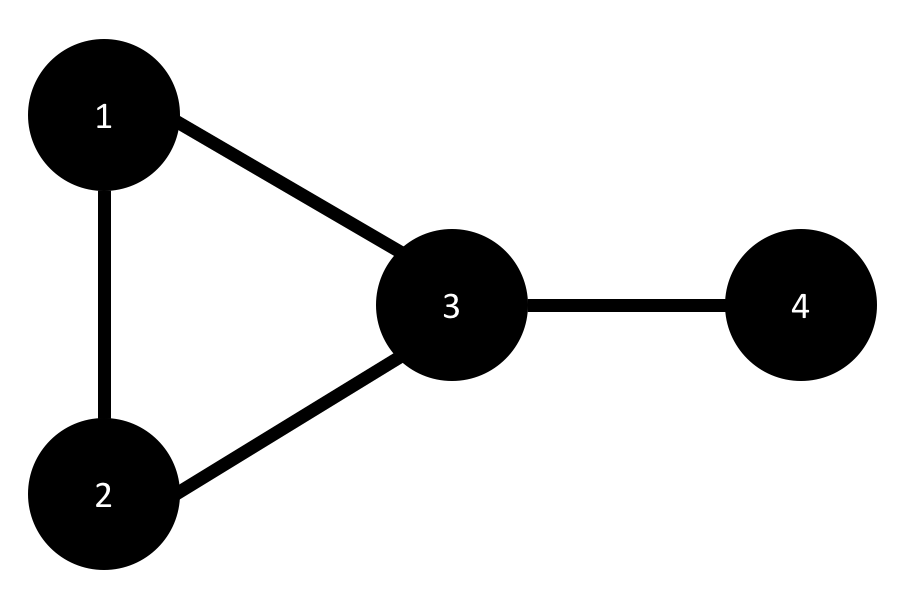
\includegraphics[width=0.6\textwidth]{fig/Paw3}
\caption{The paw graph}
\label{fig:paw3}
\end{figure}

\begin{figure}
\centering
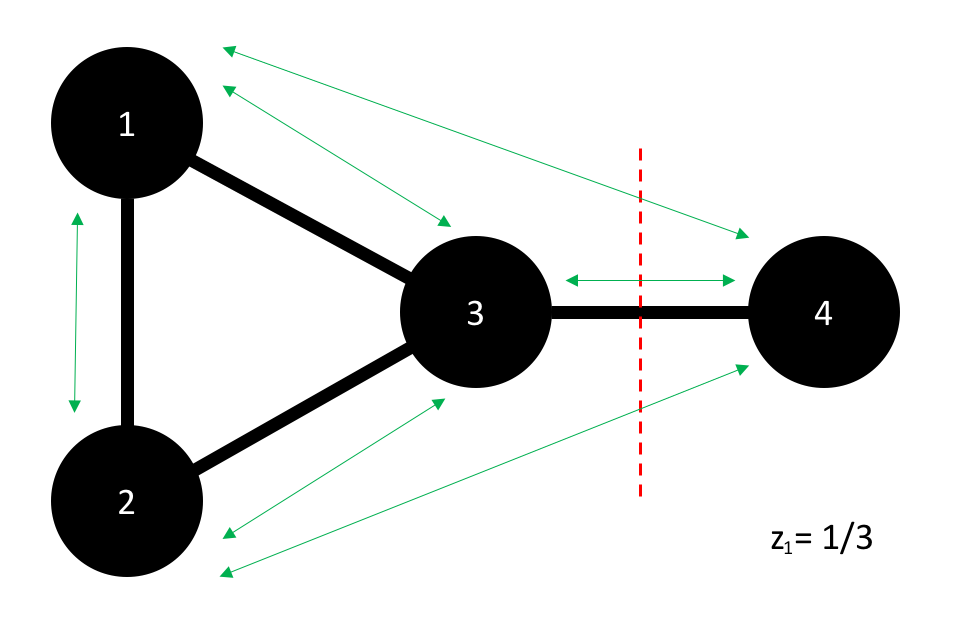
\includegraphics[width=0.6\textwidth]{fig/level1}
\caption{The first cut of the paw graph by the leximin algorithm. Green lines indicate paths of flow to fairly maximize minimum throughput. The red line indicates the cut.}
\label{fig:level1}
\end{figure}

\begin{figure}
\centering
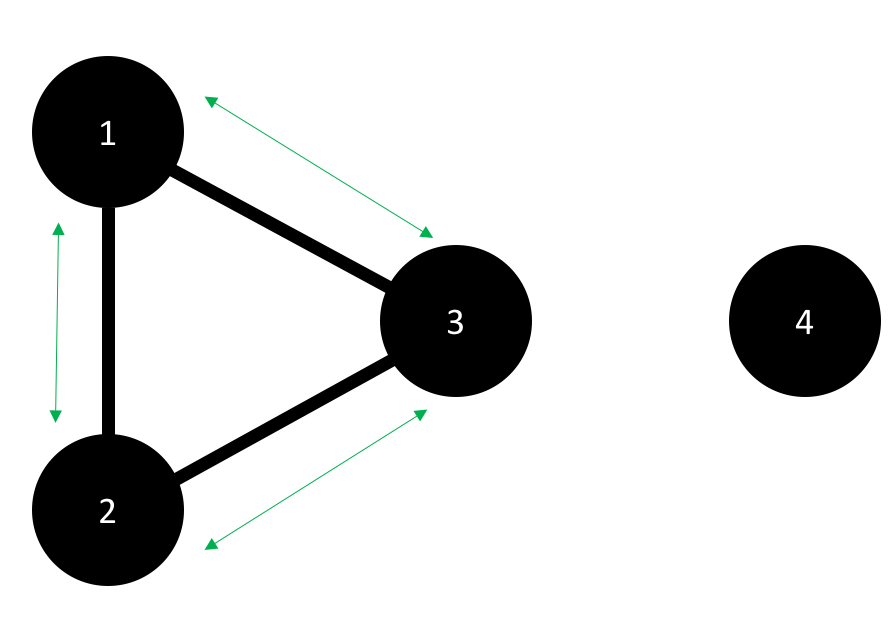
\includegraphics[width=0.6\textwidth]{fig/MCF_level2}
\caption{The subproblems for the MCF cut algorithm after its first cut: $K_3$ and a singleton}
\label{fig:MCF_level2}
\end{figure}

\begin{figure}
\centering
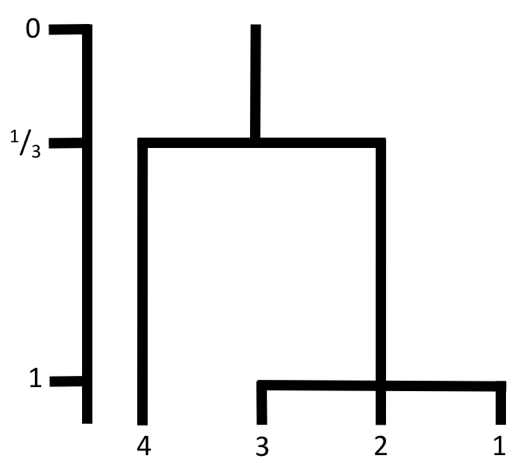
\includegraphics[width=0.4\textwidth]{fig/dendrogram_4_tie}
\caption{The dendrogram produced by the MCF cut algorithm on the paw graph}
\label{fig:MCF_dendrogram}
\end{figure}

\begin{figure}
\centering
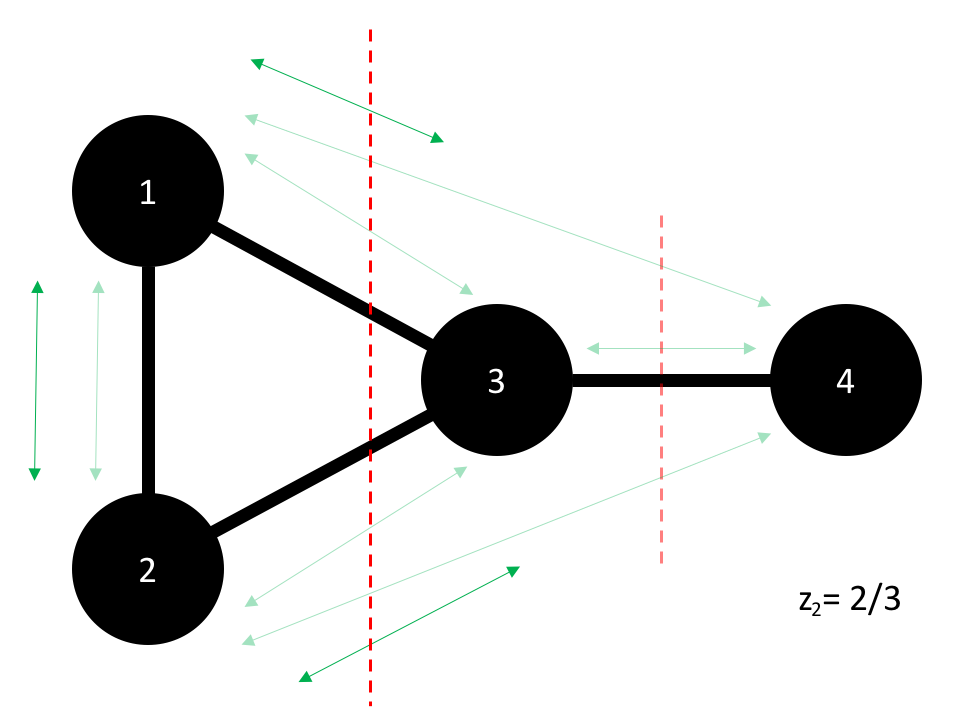
\includegraphics[width=0.6\textwidth]{fig/level2}
\caption{The second cut of the paw graph by the leximin algorithm. Green lines indicate paths of flow to fairly maximize minimum throughput. Red lines indicate cuts. Lighter colors represent fixed flow and previous cuts.}
\label{fig:level2}
\end{figure}

\begin{figure}
\centering
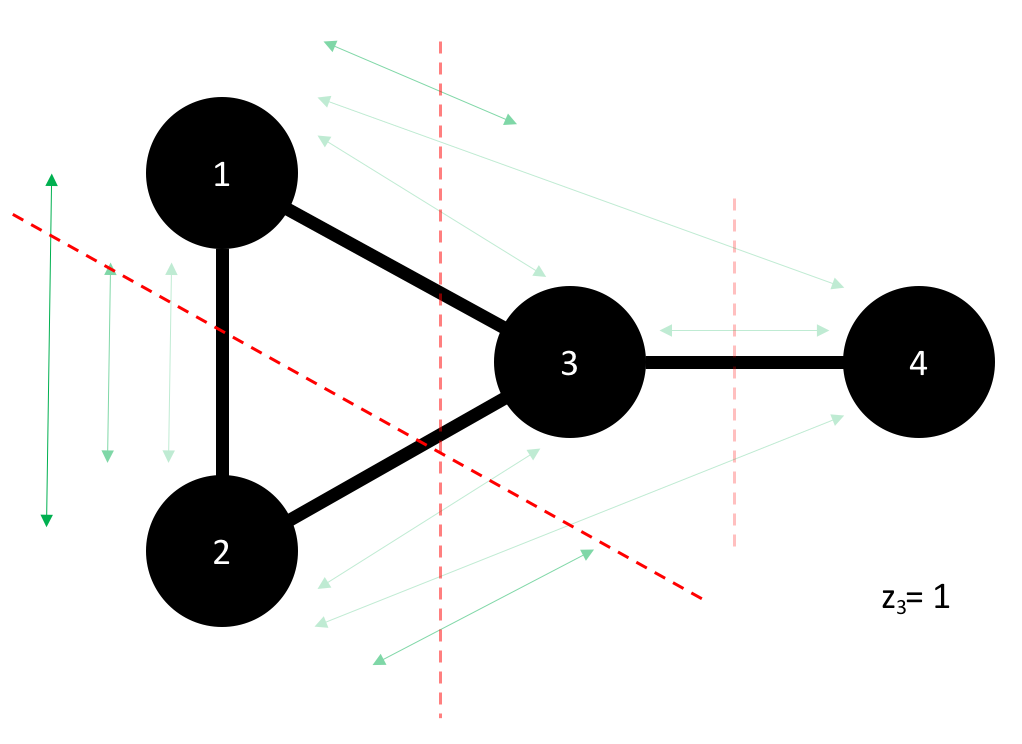
\includegraphics[width=0.6\textwidth]{fig/level3}
\caption{The third and final cut of the paw graph by the leximin method. The decision to cut $\{2, 3\}$ again instead of $\{1, 3\}$ is arbitrary.}
\label{fig:level3}
\end{figure}

\begin{figure}
\centering
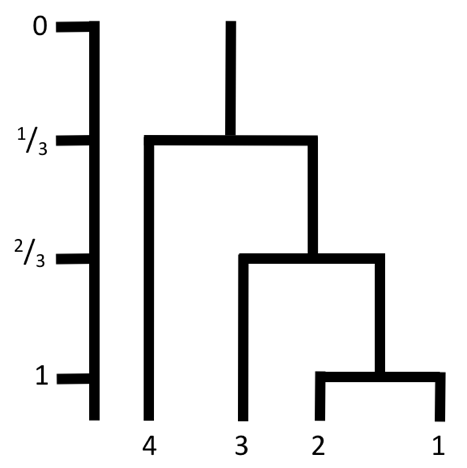
\includegraphics[width=0.4\textwidth]{fig/dendrogram_4_cascade}
\caption{The dendrogram produced by the leximin method on the paw graph}
\label{fig:leximin_dendrogram}
\end{figure}

The MCF cut algorithm is a similar technique to the leximin method which takes a divide-and-conquer approach~\cite{mann2008extensions}. It solves the MCFP on the network, then splits the network into components to process separately. This amounts to progressive filling up to the first bottleneck, then blocking the saturated pipes, draining the sections on each side, and starting anew on each side of the bottleneck. The components separated by the cut are re-solved independently of one another. This makes each subproblem smaller, but yields a different sequence of cuts and a different dendrogram.

The difference in behavior of the leximin and MCF Cut methods is best shown on a simple example. The paw graph is a graph formed by adding a fourth node to the complete graph $K_3$ and joining it to one of the existing vertices by an edge, as shown in \autoref{fig:paw3}.

The operation of the two algorithms begins identically; they differ in their treatment of subsequent steps. First, they progressively fill the network until an edge is saturated. Because this is the first iteration, there are no prior capacity usages in the leximin's hierarchical MCFP. This makes it equivalent to the MCFP solved in the MCF cut algorithm. \autoref{fig:level1} shows that the edge $\{3, 4\}$ (the \say{tail} of the paw graph) is saturated first, when there is $1/3$~unit of flow between all pairs. This edge is identified as critical. This is where the behavior deviates.

The MCF cut algorithm separates this graph into two subproblems: a triangle ($K_3$) and a singleton, as shown in \autoref{fig:MCF_level2}. When processing the triangle, we start from an initial state of no flow. Although the edge $\{1, 2\}$ had the least flow on it at the end of the first step, it is on equal footing with the other two edges of the triangle. The dendrogram for this method is then shown in \autoref{fig:MCF_dendrogram}.



In contrast to the MCF cut method, the leximin method does not remove flow already present in the network due to previous iterations. The starting point for the second iteration is shown in \autoref{fig:level2} as the lighter-colored lines. The flow required to saturate a new set of critical edges is shown in darker green. Here, there is an unambiguous next cut. The final edge is cut in \autoref{fig:level3}, which gives the final dendrogram: \autoref{fig:leximin_dendrogram}.

Because there is no clear definition of a community---and much less, a hierarchical communty---it is unclear which of these results is preferable. The leximin method has a clearer real-world significance, though: it partitions the graph based on the load applied to the graph. Further, the leximin method has desirable theoretical properties discussed in \autoref{ch:robustness}.


\section{Complexity and Size Considerations} \label{sec:complexity and size}

%The leximin algorithm is dramatically slower than competing algorithms, which can process networks with tens and hundreds of millions of nodes. The bulk of the mathematical effort  is solving the hierarchical MCFP. Proposals to increase this step's efficiency have been proposed. Dong et al.\ present the \say{triples} formulation of the MCFP, which drastically reduces the number of variables over the edge--path formulation, while also reducing the number of constraints~\cite{dong2015compact}.  Nevertheless, a dense network of 160 nodes can take an hour to process on current hardware. 

Solving a linear program is a polynomial-time technique, when inputs are algebraic numbers~\cite{adler1992polynomial}. The fastest known LP method has complexity $$O\left(\frac{n^3}{\log n}L\right)$$ where $n$ is the number of variables in the standard form of the LP and $L$ is the information length of the LP, which grows with the product of the number of variables and constraints~\cite{anstreicher1999linear}. In the efficient \say{triples} formulation of the MCFP, there are $O(mN)$ variables and $O(N^2)$ constraints. 

Since real-world networks have sparse connectivity~\cite{chakrabarti2006graph}, we can restrict our focus to these. Even on sparse graphs, solving an LP will take essentially $O(N^{10})$ time relative to the number of nodes in the graph. Given that up to $(N-1)$ LPs will be solved (one for each level of the hierarchy~\cite{nace2003some}), this amounts to a complexity of near $O(N^{11})$. The next slowest options are Walktrap ($O(N^{3.2})$) and Girvan--Newman ($O(N^3)$ on sparse graphs). 

\subsection{Practical Considerations for Implementation}
The edge--path form of the MCFP involves an exponential number of variables, which is untenable. Fortunately, more efficient representations have emerged. An implementer should prefer the triples formulation of the MCFP~\cite{dong2015compact}, which is easily extended to the hierarchical case. This method has a polynomial number of variables and constraints, yielding a tractable linear program in the complexity class P\@. Work to expedite handling degenerate cuts has also been done~\cite{danna2012practical}. The details of such a method, as well as its implementation, are out of the scope of this work.

Additionally, the method should only be applied to graphs of up to a few hundred nodes. On a sparse graph of 240 nodes, the runtime is measured in hours.

%\begin{algorithm}
%	\caption{MCF cut algorithm~\cite{mann2008extensions}}
%	\label{alg:mcf_cut}
%		\KwData{A graph $G = (V, E)$, edge capacities $c$, demand pairs $d$}
%		\KwResult{A clustering $\mathcal{C}(G)$}
%		$queue \longleftarrow \{G\}$
%		\While{$queue \neq \emptyset$}{
%			$H \longleftarrow queue.dequeue()$\;
%			\textbf{Solve the MCFP on $H$}\;
%		    Extract critical edges~$\hat{E}_i$: those with nonzero shadow prices \;
%		    \Unless{Something}{
%			\ForEach{component $H_j$ in $H$ cut by $\hat{E}_i$}{
%				$queue.enqueue(H_j)$\;
%			}}
%		}
%		\vspace{0.25cm}
%\end{algorithm}

   
   \chapter{ROBUSTNESS OF MCF CUT ALGORITHM} \label{ch:robustness}% Must have a blank line after every section label

\section{Introduction} \label{sec:robustness introduction} % Must have a blank line after every section label

\say{Standard form} is the usual and most intuitive form of describing a linear programming problem. It consists of the following three parts:
\begin{itemize}
\item A linear \say{cost} function to be minimized
e.g. $ z(x_{1},x_{2}) = c_1 x_1 + c_2 x_2$
\item Problem constraints of the following form, e.g.
\begin{equation}
\begin{matrix}
  a_{11} x_1 + a_{12} x_2 &\geq b_1 \\
  a_{21} x_1 + a_{22} x_2 &\geq b_2 \\
  a_{31} x_1 + a_{32} x_2 &\geq b_3 \\
\end{matrix}\end{equation}
\item Non-negative variables, e.g.
\begin{equation}\begin{matrix}
 x_1 \geq 0 \\
 x_2 \geq 0
\end{matrix}\end{equation}
\end{itemize}

The problem is usually expressed in matrix form, and then becomes:
\begin{equation}
\min \{ %
\mathbf{c} \transpose
\mathbf{x} \;|\;
 A \mathbf{x} \geq \mathbf{b} \land \mathbf{x} \geq 0 \}
\end{equation}

\subsection{Sensitivity} \label{sec:sensitivity}

Every linear program has a corresponding dual program in the form:

\begin{equation}
\min \{ %
\bm{\lambda} \transpose
\mathbf{b} \;|\;
\bm{\lambda} \transpose A \geq \mathbf{c} \transpose \land \bm{\lambda} \geq 0 \}
\end{equation}

The solutions to the dual program provide \say{shadow prices}, which give a range of values over which the solution is optimal.

Small changes to $\mathbf{b}$ will not change the optimal basis, and there is a linear relationship between the change $\Delta \mathbf{b}$ and the change in the objective $\Delta z$.

\section{Experiments} \label{sec:robustness experiments}

Why you can use multigraph and/or variable capacity.

\subsection{Triangle} \label{sec:triangle}

\subsection{Bridges of K\"onigsberg}

\begin{figure}
\centering
\begin{minipage}{0.45\linewidth}
\centering
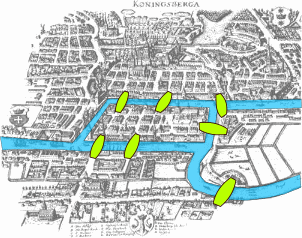
\includegraphics[width=\textwidth]{fig/bridges_map}
\end{minipage}
\begin{minipage}{0.45\linewidth}
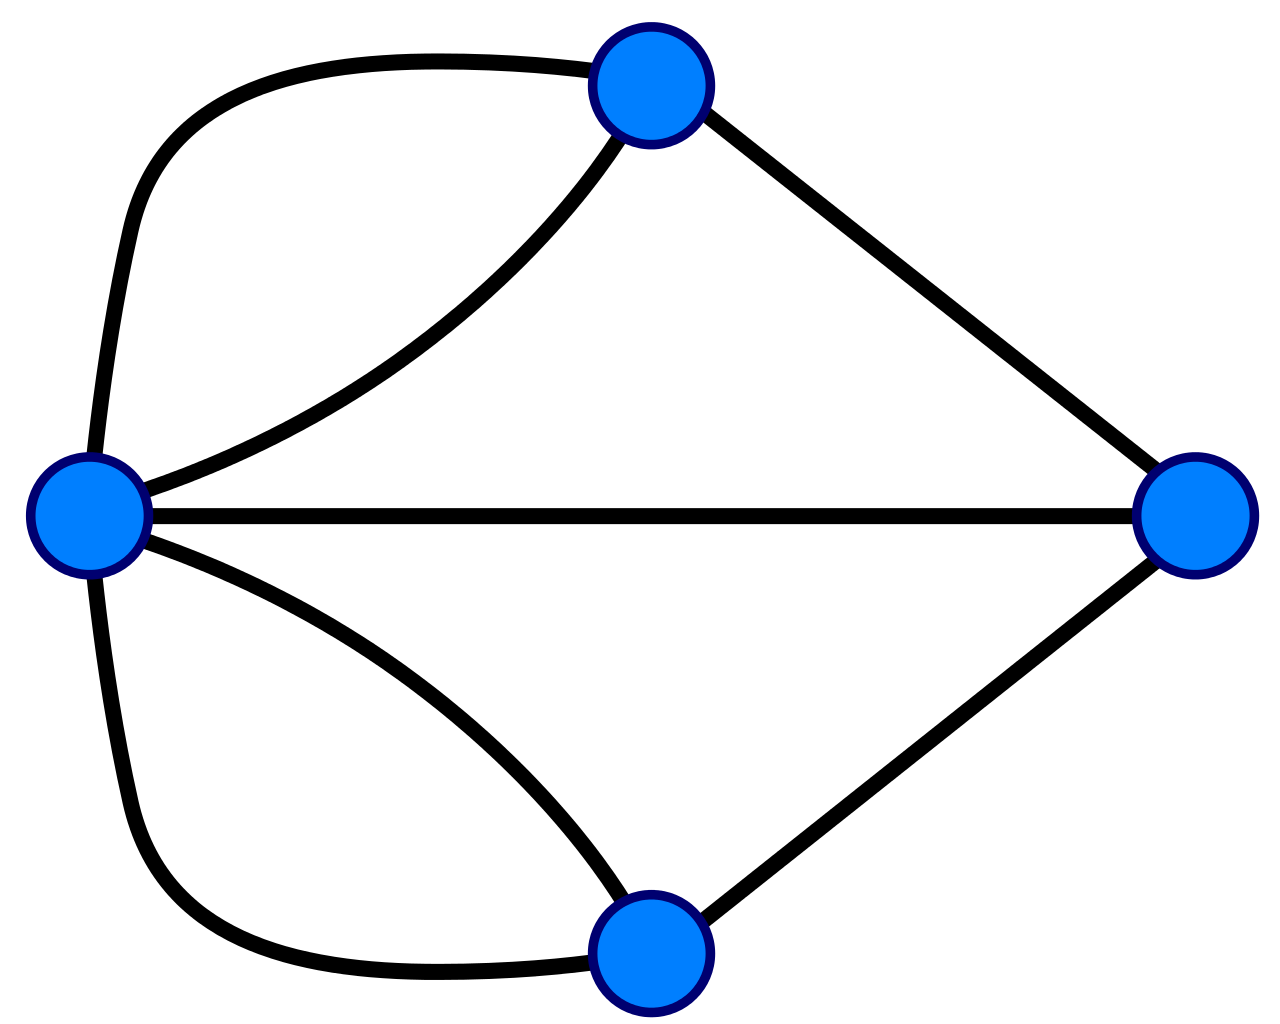
\includegraphics[width=\textwidth]{fig/bridges_graph}
\end{minipage}
\caption{The bridges of K\"onigsberg, as a map and a multigraph}
\label{fig:bridges}
\end{figure}

The bridges of K\"onigsberg spawned the traveling salesman problem (TSP) and what is seen as the first proof in the field of network science~\cite{newman2003structure}. The graph (shown in \autoref{fig:bridges}) is an illustrative example of the 

\subsection{K\textsubscript{3,2}}

\subsection{Florentine families}

   
   \chapter{RANDOMNESS AND GRIDLOCK} \label{ch:random}

\epigraph{Everything we care about lies somewhere in the middle, where pattern and randomness interlace.}{James Gleick, \emph{The Information: A History, a Theory, a Flood}}

In this chapter, I define and examine the \emph{gridlock} behavior of the leximin method. In the case of random graphs, I show a reliable tendency that for some edge creation probability $p$, as the network size grows, the occurrence of gridlock becomes more frequent. I show that for any gridlock graph with rational capacities, there exists a constant $k$ such that when the capacities of all edges are $k$, integer flows can be assigned along each path. For diameter-2 random graphs, I conjecture that this value $k$ is $M / [N (N-1) - M]$.





\section{Introduction}

If a community detection method splits a global community into all individuals, and the method has some justification as realistic, then this behavior says that the input is indistinguishable from what random associations would give. Only two levels of structure exist: the macroscopic level of the entire graph and the microscopic level of single nodes. There is no mesoscopic, community structure.

The leximin method for community detection has a tendency to produce the microscopic structure as the only partition in its hierarchy under certain conditions. We call this phenomenon \emph{gridlock}. When it occurs, we affirm that a particular example is \emph{practically} equivalent to random associations. This may suggest that methods which generate hierarchies on these networks lack the causality to do so; instead, they overzealously force communities to be generated in the given example. Obtaining a hierarchy inexplicable by causality is at best problematic and effectively accidental. 

\subsection{Gridlock}

The only replicable partition, irrespective of a random edge creation process, is immediate separation into individual singleton parts. The leximin method can identify such a partition into communities as the only extant one, because every edge is saturated simultaneously. This is \emph{gridlock}. Only the macro- and microscopic structure exist, without a mesoscopic structure. A graph with these properties is called a \emph{gridlock graph}.

What differentiates gridlock from a tie is the width of the stable ranges. In a tie, the stable ranges are tight because ties straddle the boundaries of two behaviors, creating a superposition of dendrogram states. By contrast, gridlock is a stable behavior. The width of the stable range along any axis is not infinitesimally small. Gridlock need not occur at the first level of the hierarchy, but in this work, we specify when gridlock is not immediate. In general, we use the term to refer to immediate gridlock.

A useful lemma about gridlock and modularity can be proven based on a lemma given by Brandes et al.~\cite{brandes2007finding}:
\begin{lemma}
\label{lemma:modularity}

A clustering with maximum modularity has no cluster that consists of a single node with degree 1.
\end{lemma}

Gridlock is a clustering with very low modularity, according to Lemma \autoref{lemma:modularity}. In fact, the modularity of singleton clustering is the minimum possible~\cite{brandes2008modularity}. This suggests a corresponding Lemma:

\begin{lemma}
\label{lemma:grids}

If the modularity-maximizing flat clustering produced by the leximin method is into singletons, then gridlock has occurred. 
\end{lemma}

\begin{proof}
According to Lemma \autoref{lemma:grids}, the singletons of gridlock produce the worst possible modularity. If they are the highest-modularity clustering found, then there exist no other clusterings in the dendrogram. 
\end{proof}

A final observation is that when immediate gridlock occurs, there is only one level in the hierarchy, so the leximin and maximin solutions are the same. Since only one level is solved, rather than up to $N - 1$, a lack of community structure causes the method to \say{fail fast}.



\subsection{Random graphs}

A helpful model to examine this structure of random connections is the binomial graph model. It produces a graph~$G(N, p)$, specifying the number of nodes~$N$ and the probability of an edge between each pair of nodes~$p$. The model was introduced by Gilbert~\cite{gilbert1959random} and analyzed by Erd\H{o}s and R\'enyi~\cite{erdos1960evolution}. 

Much attention has been given to the problem of a dense community \emph{planted} in an otherwise random graph~\cite{hajek2015computational, arias2013community}. Less attention has been given to the \emph{existential} problem of communities in random graphs---of structure inherent in randomness. An exception to this is what has been called \say{one of the most surprising results in the theory of random graphs}: the identification of a reliable largest clique size for a given $p$~\cite{matula1976largest, palmer1985graphical}. Although the largest clique size is replicable across instances of the random graph with given parameters, the particular set of members is almost certainly not replicable. The issue of determining a well-defined cluster of members that should recur is not affected by this observation. Additional work has been done to identify communities in random graphs by consensus using nondeterministic methods~\cite{campigotto2013power} and to relate community size in random graphs to component size~\cite{lipowski2014generic}.

To assess whether there exists a community structure in random graphs, we use the leximin method. For a sufficiently homogeneous graph, the leximin method exhibits gridlock. As the first and only possible partition, it separates the graph into singletons. This dissection suggests a lack of mesoscopic, community structure in the graph. Computational results presented below support this conclusion.





\section{Experimental Evidence} \label{sec:random_experiment}

\begin{figure}
\centering
\begin{subfigure}[c]{0.48\textwidth}
\centering
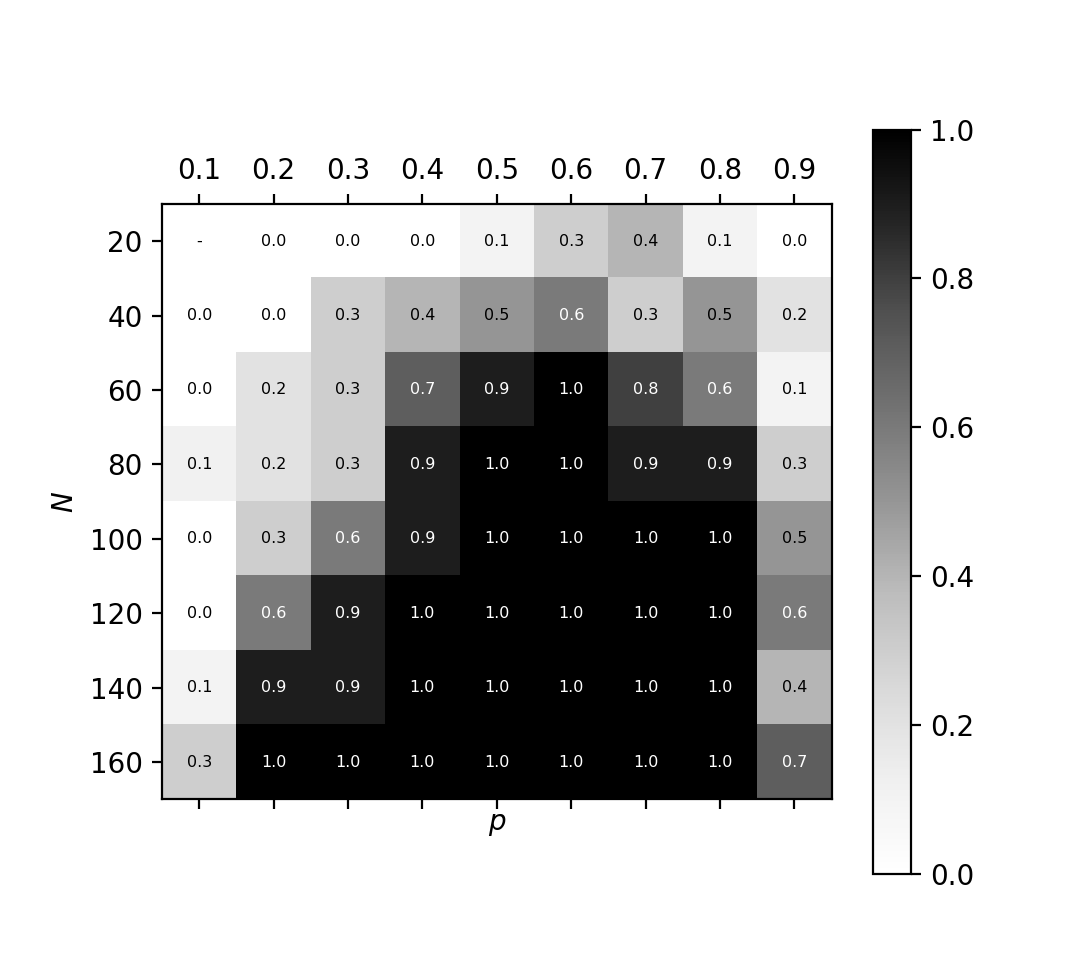
\includegraphics[height=0.225\textheight]{fig/gridlock_big}
\caption{Group 1: 10 trials each}
\end{subfigure}
\quad
\begin{subfigure}[c]{0.48\textwidth}
\centering
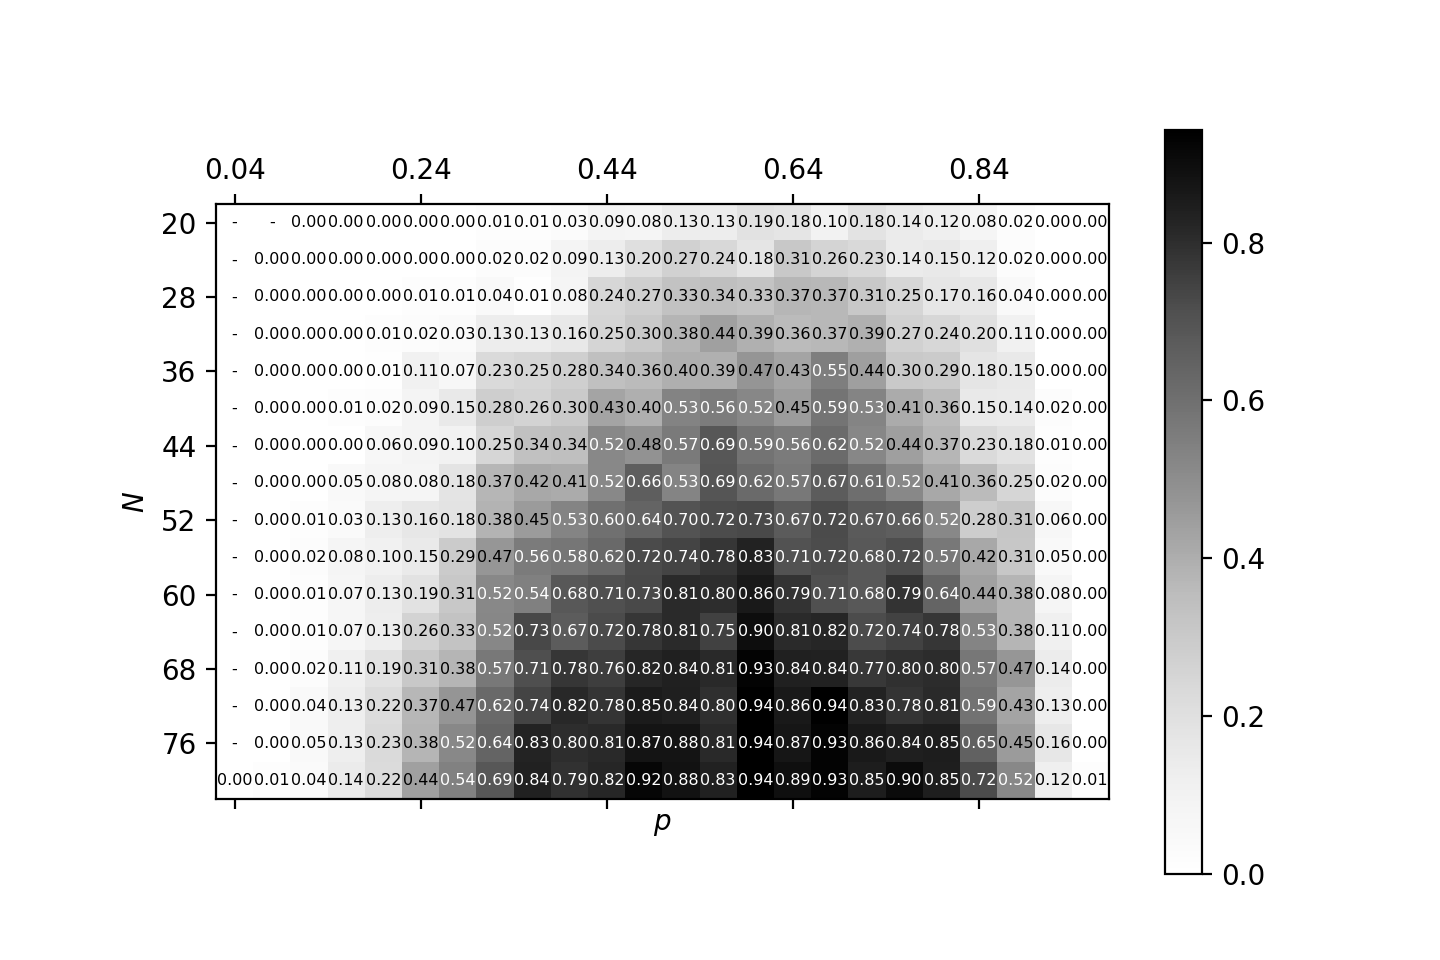
\includegraphics[height=0.225\textheight]{fig/gridlock_small}
\caption{Group 2: 100 trials each}
\end{subfigure}
\caption{Rate of gridlock for each combination of $N$ and $p$}
\label{fig:gridlock}
\end{figure}

To examine the community structure of random graphs, two groups of test graphs were created:
\begin{description}
\item[Group 1.] 10 graphs each at $N = 20, 40, \ldots, 160$ and $p = \frac{1}{10}, \frac{2}{10}, \ldots, \frac{9}{10}$
\item[Group 2.] 100 graphs each at $N = 20, 24, \ldots, 80$ and $p = \frac{1}{25}, \frac{2}{25}, \ldots, \frac{24}{25}$
\end{description}
For each of these parameter combinations, we computed the fraction which display immediate gridlock. From the empirical results shown in \autoref{fig:gridlock}, we see a tendency that for a given $p$, increasing $N$ reliably increases the rate of immediate gridlock.

It is important to note that middle values of the edge probability~$p$ are capable of producing gridlock at lower sizes~$N$, compared to high or low values. For lower values, the reason is that so few edges naturally impart a structure; after all, there is a threshold $p = 1/n$ for the graph to be connected at all~\cite{frieze2015introduction, janson2011random}. On the higher end, gridlock is less common because removing edges from a complete graph (i.e.\ one with $p=1$) produces nodes of minimum degree less than $N - 1$. The resulting asymmetry of node degree generally yields more than one level in the leximin hierarchy. This investigation of the number of levels and the causes is worthy of more investigation.





\section{Discussion}

We can show a result for maximum concurrent flow similar to Menger's theorem for maximum flow~\cite{menger1927allgemeinen}: that a multigraph of the gridlocked graph exists where all edges can be partitioned into edge-disjoint paths with the same number of paths between each node pair.

\begin{theorem}{Edge-disjoint paths in gridlock graphs.} \label{thm:edge}


A multigraph of the gridlocked graph exists where all edges can be partitioned into edge-disjoint paths with the same number of paths between each node pair.
\end{theorem}
\begin{proof}
In a gridlock graph, the demand between all pairs is equal, and the utilized capacity of each edge is equal. The flow may be diverted between various intermediate nodes before reaching its destination, possibly taking multiple paths.

Linear programs with integer coefficients (like the HMCFP) produce rational results~\cite{adler1992polynomial}, so the flow assigned to each path will be rational: a value $p/q$ where $q \ne 0$. Let $k$ be the least common multiple (LCM) of all the denominators of the flows on each path. Assigning this value as the capacity of each edge creates integer-valued flow along all paths, indicating the number of copies of each path. This also means that the capacity of an edge is split into integral flows, from each path that uses that edge.

Each capacitated (weighted) edge with capacity $C$ can be replaced with $C$ unweighted edges, producing the desired multigraph. A path that requires $c < C$ units of flow can utilize $c$ of the $C$ edges. All paths will do this, resulting in edge-disjoint paths on the multigraph. 
\end{proof}

An example application of this theorem is the smallest nontrivial graph with gridlock: $K_{3,2}$. Its throughput is $z = M/[N (N -1) - M] = 6/14 = 3/7$. The flow allocations on each path have denominators of 7 or 14. When scaling up all flows by the LCM of these values, we get 14 unweighted paths between each pair. \autoref{fig:k32_integer} shows the unweighted multigraph's edge-disjoint paths.

\begin{figure}
\centering
\begin{subfigure}[c]{0.48\textwidth}
\centering
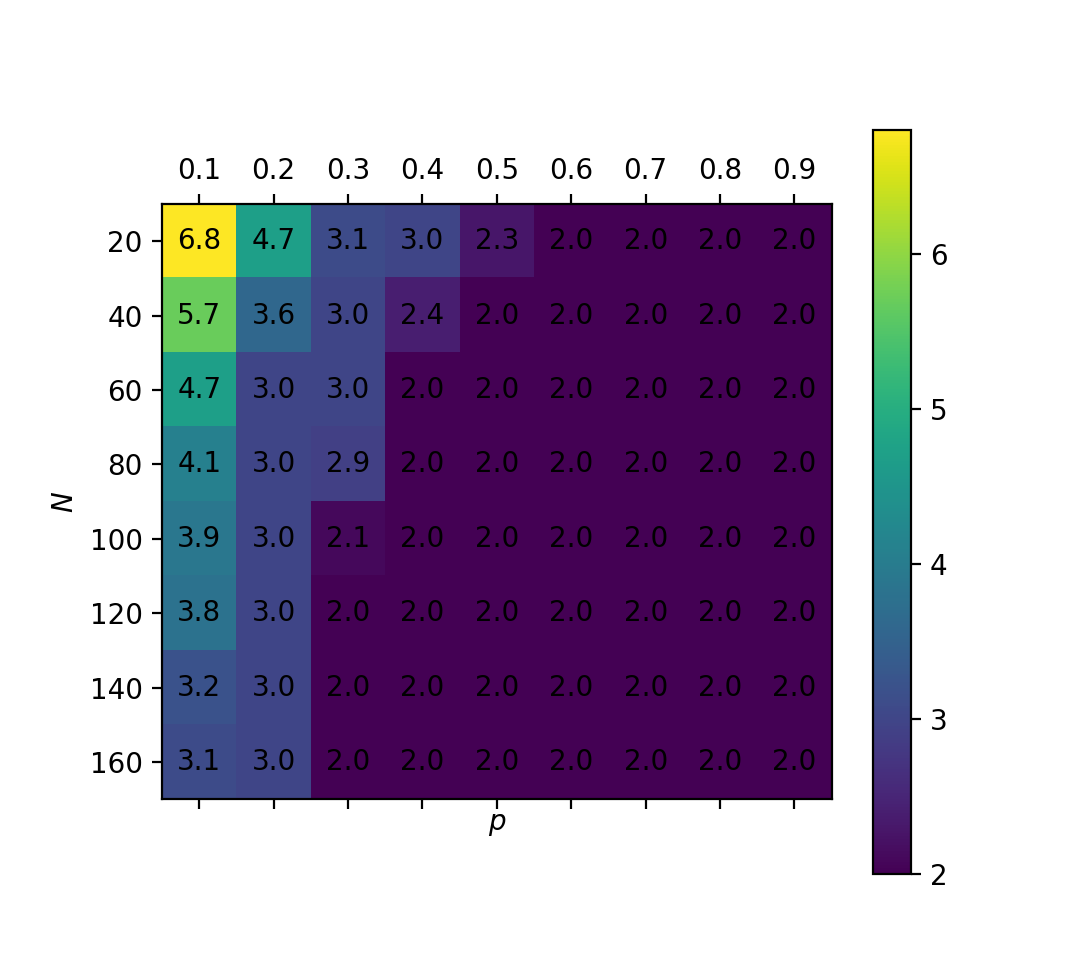
\includegraphics[height=0.225\textheight]{fig/diameter_big}
\caption{Group 1: 10 trials each}
\end{subfigure}
\quad
\begin{subfigure}[c]{0.48\textwidth}
\centering
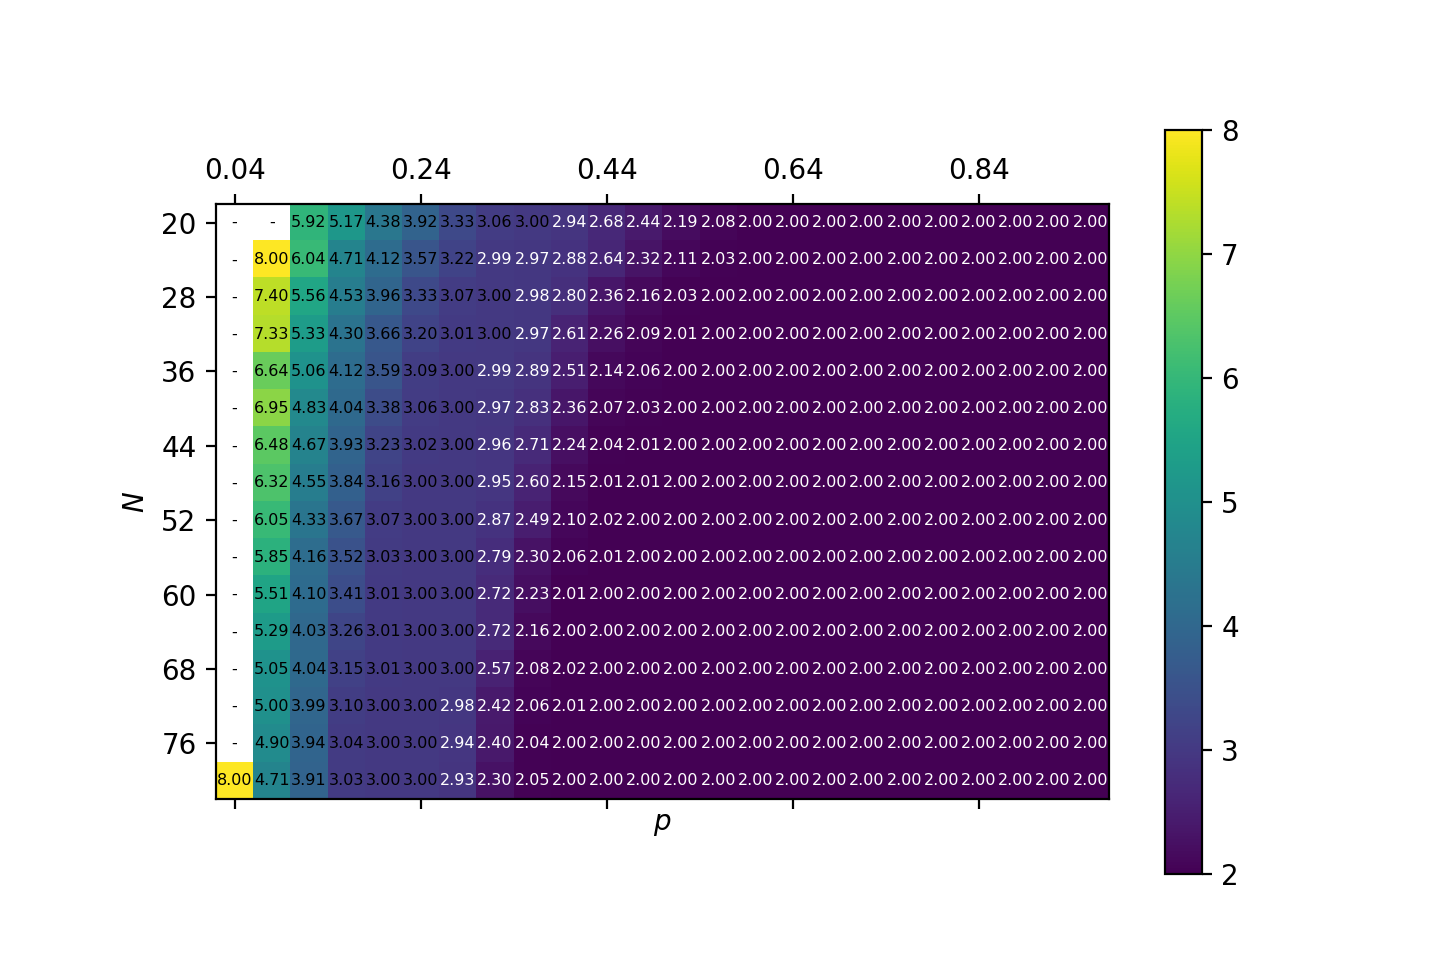
\includegraphics[height=0.225\textheight]{fig/diameter_small}
\caption{Group 2: 100 trials each}
\end{subfigure}
\caption{Average diameter for each combination of $N$ and $p$}
\label{fig:diameter}
\end{figure}

\begin{figure}
\centering
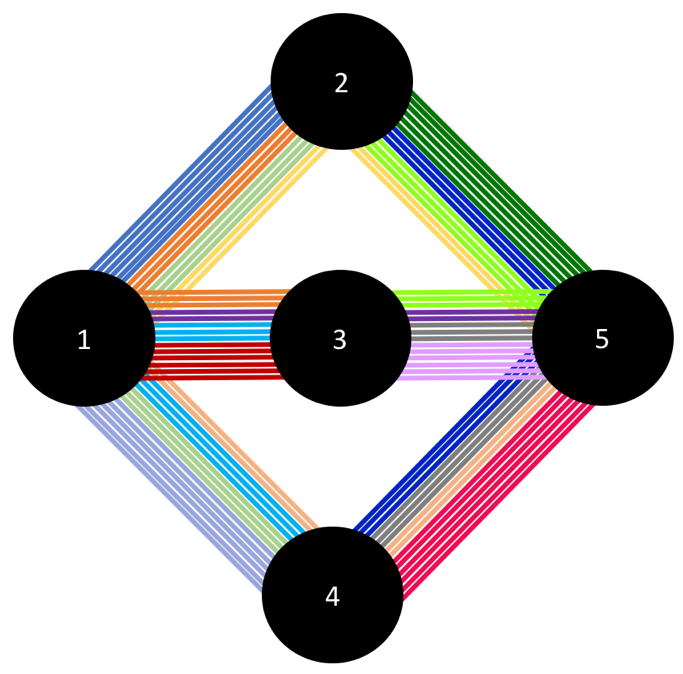
\includegraphics[height=0.25\textheight]{fig/k32_integer}
\caption{The gridlock graph $K_{3,2}$ represented as a multigraph. A single color corresponds to a single route. There are $[N (N-1) - M] = 14$ edges between each node, and 6 are used for demand between each pair of nodes. 2 units between the end nodes 1 and 5 are routed through each middle node 2, 3, and 4. 3 units between each pair of middle nodes are routed through each end node.}
\label{fig:k32_integer}
\end{figure}




\subsection{Gridlock Graphs with Diameter 2}

In the experiment from \autoref{sec:random_experiment}, most graphs that gridlock have diameter 2 (see \autoref{fig:diameter}). This is not a requirement; we see from the $(N=160, p=0.3)$ case that gridlock is possible on a diameter-3 graph (see \autoref{fig:diameter}).

In the case that the diameter is 2, the maximum throughput is easily computable. There exist $|D| = {N \choose 2}$ demand pairs, of which $M$ are at distance 1. Thus, the sum of all shortest path lengths is $M + 2(|D| - M) = 2|D| - M$. These shortest paths must carry all flow, or else we waste capacity by taking longer paths~\cite{mann2008extensions}. Additionally, because we assume unit capacity on each edge, the total capacity is $M$. The throughput is then $z = M / [N (N-1) - M]$. This is the \emph{gridlock bound}, first identified by Biswas and Matula~\cite{biswas1986two}. 

Since throughput is the amount of flow between each pair, we can get an integral flow of $M$ units when we scale up the capacity of each edge by the denominator $[N(N-1)-M]$. 

We can consider specific cases of diameter-2 gridlock graphs with low $p$, with scaled-up edge capacity. These tend to produce several paths at integral flow $M$, as well as some paths with either integral or  fractional values that sum to $M$. We know these values are fractional, rather than irrational, because linear programs with integer coefficients produce rational results~\cite{adler1992polynomial}. The question emerges whether there exists an assignment of flow that is not only rational, but also integral.

\begin{description}
\item[Conjecture.] \emph{In a random graph of diameter 2 and $p<0.5$ that exhibits gridlock, there exists an integer assignment of flows to paths when the capacity of edges is equal to $[N ( N - 1 ) - M ]$.}
\end{description}

As a justification for this conjecture, consider the fact that there exists a multiple of $[N ( N - 1 ) - M ]$ where all paths have integer flow. This comes from Theorem \autoref{thm:edge}. Additionally, the case of $K_{3,2}$ did evenly split its flow along integer paths, as shown in \autoref{fig:k32_integer}. What remains is to show that this multiple is in fact exactly $[N ( N - 1 ) - M ]$ in all such cases.

More work is needed here to prove the conjecture provided above, or to otherwise determine how big the edge multiplicity must be, such that it prescribes a partition into paths with the same number of paths between each node pair. A major hindrance is that while a unique set of critical edges exists, there is not necessarily a unique assignment of flow along paths. To guarantee an integer solution (if it exists) is possible using integer linear programming (ILP), which is NP-hard.



   \chapter{COMPARISON WITH POPULAR METHODS} \label{ch:comparison}% Must have a blank line after every section label

\section{Introduction} \label{sec:comparison introduction}

\subsection{Hierarchical clustering}\label{sec:Hierarchical Clustering}

\subsection{Flat cluster extraction}\label{sec:Flat Cluster Extraction}

Once the dendrogram structure relating nodes has been identified, one must extract a set of flat (i.e. non-nested) clusters. Informally, this is often done by drawing a horizontal line across the dendrogram: the clusters which this line crosses are selected. Other methods exist which can adaptively select cluster groups, especially when a minimum cluster size is specified~\cite{campello2013density}.

The popular metric for deciding at which level to cut is Newman's modularity score, $Q^W$~\cite{newman2006modularity}. As Mann notes, others exist; he relies on maximizing average degree. \todo{Beware: Limits of modularity maximization in community detection by Fortunato...}

\subsection{Mixing coefficient ($\mu$)}

\subsection{LFR benchmark} \label{sec:LFR Benchmark} % Must have a blank line after every section label

Mann tested on the GN benchmark, which has these problems: x, y, z.

This parameterization of the model largely aligns with the work of Yang et al.~\cite{yang2016comparative}. Due to the temporal constraints of the MCF algorithm, the average degree and network size parameters needed to be reduced. The community size and degree distribution exponents are preserved at -1 and -2 respectively, as discussed in Lancichinetti et al.~\cite{lancichinetti2008benchmark}.

\begin{table}
	\centering
		\begin{tabular}{l r}
		\toprule
		Parameter & Value \\
		\midrule
		Number of nodes $N$ & 10--150 \\
		Maximum degree & 0.2N \\
		Maximum community size & 0.1N \\
		Average degree & 10 \\
		Degree distribution exponent & -2 \\
		Community size distribution exponent & -1 \\
		Mixing coefficient $\mu$ & [0.03, 0.75] \\
		\bottomrule
		\end{tabular}
	\caption{Parameter grid for LFR benchmark graphs}
	\label{tab:Parameter grid}
\end{table}

\subsection{Evaluating quality of clustering}

Mann proposed a metric $M$ for scoring the partition of a network into communities. Objecting to the use of vertex set membership metrics, he proposed to use the accuracy score of a binary classification of edges as inter- or intra-community edges. He used this evaluation to show the superiority of the MCF algorithm over the edge betweenness algorithm of Girvan and Newman, which repeatedly removes the most \say{between} edge, potentially removing edges within an identified cluster. As the MCF algorithm cannot remove an edge within a community\todo{Do I need to prove this?}, the edge betweenness algorithm can receive a lower score while identifying the same communities. Further, the $M$ score's \say{sensitivity} to edges is irrelevant in other techniques which do not rely on edge removal. The metric seems specifically tailored to penalize the edge betweenness algorithm.

Here, the normalized mutual information metric~\cite{danon2005comparing} and the ratio of detected to true clusters~\cite{yang2016comparative} are used. 

\section{Results}\label{sec:comparison results}

< Show one LFR benchmark, clustered by ground truth and then by our method. >

< Also show the dendrogram for our method. >

Three factors prevent us from adequately comparing the runtime of the MCF algorithm to the other clustering techniques. Most importantly, the implementation of the MCF algorithm does not perform a \say{warm start}: at each level, rather than restarting at the previous solution, it starts at the base initialization again. This inflates the actual runtime relative to an ideal implementation. Second, the algorithms are implemented in different languages. The \texttt{igraph} package is implemented in C with interfaces to Python and R, whereas the MCF algorithm is written in AMPL.


%   \chapter{INSULARITY AS A MEASURE OF NETWORK ROLES} \label{ch:insularity}% Must have a blank line after every section label

\section{Introdution} \label{sec:insularity introduction} % Must have a blank line after every section label

Insularity is computed from the LP in a manner similar to Mann's computation of flowthrough centrality; however, it is a dynamic property of the network: a function of the network's utilization. 

Flowthrough centrality is computed by solving the HMCFP to the point of total saturation; it is related to the node's the node's capacity (its weighted degree, a property of the graph) and the amount of flow terminating at that point, which is given in the solution of the HMCFP. 

\section{Results}

Stuff

%   \chapter{RESULTS} \label{ch:results}% Must have a blank line after every section label
        %  2. Chapter 2
   
   \chapter{CONCLUSION} \label{ch:conclusion}% Must have a blank line after every section label

Summary of the problem, the main findings and the discussion. Structured according to the issues in Related Literature and Theoretical Focus.

Comparison with the literature: how do your results fill in, advance or contradict previously reported research?

What are the implications of your research for people working in the field that you have studied?

In which direction should further research go?

\section{Overview of Significant Research Results} \label{sec:Overview} % Must have a blank line after every section label

\section{Comparison to Popular Methods}

\section{Sensitivity and Robustness}

\section{The Insularity Measure}

\section{Future Work}



%-----------------------------------------------------------
%   Appendices go here if no appendix, remove \StartAppendix
%-----------------------------------------------------------
   \StartAppendix           %  All chapters from this point are treated as appendices
   
   \chapter{RELEVANT BACKGROUND IN LINEAR PROGRAMMING} \label{app:LP}% Must have a blank line after every section label

This appendix presents an operational description of linear programming (LP), a method of constrained optimization for linear systems of inequalities. Linear programs are the common method for solving the maximum concurrent flow problem (MCFP) and hierarchical MCFP (HMCFP). For greater detail, the reader is directed to Luenberger and Ye~\cite{luenberger2008linear} or Chvatal~\cite{chvatal1983linear}.

\section{Linear Programming}

Linear programming optimizes an objective function that is constrained by linear equalities and inequalities. For some linear objective function $z = c \transpose x$, we want to find the $x$ that maximizes $z$ while constrained by a system of linear inequalities $Ax \leq b$. 

A linear program in standard form comprises three parts:
\begin{enumerate}
\item A linear \say{cost} function to be maximized, e.g. $ z(x_{1},x_{2}) = c_1 x_1 + c_2 x_2$
\item Problem constraints, e.g.
\begin{equation}
\begin{matrix}
  a_{11} x_1 + a_{12} x_2 &\leq b_1 \\
  a_{21} x_1 + a_{22} x_2 &\leq b_2 \\
  a_{31} x_1 + a_{32} x_2 &\leq b_3 \\
\end{matrix}\end{equation}
\item Non-negative variables, e.g.
\begin{equation}\begin{matrix}
 x_1 \geq 0 \\
 x_2 \geq 0
\end{matrix}\end{equation}
\end{enumerate}
Problems with equality constraints or bounds other than non-negativity can be converted into these three parts; the reader is directed toLuenberger~and Ye~\cite{luenberger2008linear}. The problem is usually expressed in matrix form, and then becomes:
\begin{equation}
\max \{ %
\mathbf{c} \transpose
\mathbf{x} \;|\;
 \mathbf{A} \mathbf{x} \leq \mathbf{b} \land \mathbf{x} \geq 0 \}
\end{equation}

These linear constraints form half-planes that bound a convex polytope (a bounded polyhedron)~\cite{nemhauser1988integer}. Any point inside this polytope is a \emph{feasible solution}. 

Solving a linear program (when a solution exists) gives an optimal basis~$\mathbf{B}$. This basis is a matrix of  For a given basis, there is a corresponding \emph{basic solution}~$(\mathbf{x_B}, \mathbf{0})$. Here, $\mathbf{0}$ is the zero vector. The solution only has values for each $x_i$ corresponding to a column in $\mathbf{B}$. At most, $m$ of its entries are nonzero, where $m$ is the number of columns in A. (Here, we assume as for our problem that the number of rows $n \geq m$. 

\section{Shadow Prices and Sensitivity}

Every linear program has a corresponding dual program in the form:

\begin{equation}
\min \{ %
\bm{\lambda} \transpose
\mathbf{b} \;|\;
\bm{\lambda} \transpose \mathbf{A} \geq \mathbf{c} \transpose \land \bm{\lambda} \geq 0 \}
\end{equation}

The solutions to the dual program provide \emph{shadow prices}~$\bm \lambda$. The shadow prices reflect the marginal utility of relaxing the corresponding constraint in the primal, or the marginal cost of tightening the constraint:

\begin{align}
\lambda_i = \frac{\partial z}{\partial b_i}, \quad \forall i \in \{1, 2, \ldots, |\lambda|\}
\end{align}

These shadow prices are piecewise linear, and the particular range over which some shadow price~$\lambda_i$ is valid can be computed~\cite{luenberger2008linear}: when a value in $\mathbf{b}$ is altered, the values of the right-hand side in the optimal tableau are altered. The stable range is the interval along which the right-hand side of the tableau remains nonnegative. 

\section{Practical Considerations}

LPs can be quickly solved using the simplex method~\cite{puterman2014markov}. Although the method scales exponentially with input size in the worst case, average-case performance is far better. Additional methods have been proposed with polynomial worst-case behavior, such as interior point methods.
          %  Appendix A

%-----------------------------------------------------------
%   Bibliography goes below
%   Check with specific department on the appropriate
%   bibliography style to use
%-----------------------------------------------------------
   \nocite{*}
   \bibliographystyle{alpha}
   \raggedright
%   \footnotesize           % For smaller font on Bibliography
   \bibliography{thesisbib}
%   \normalsize             % Uncomment to return to normal font after smaller font

%-----------------------------------------------------------
%   END body of the thesis
%-----------------------------------------------------------
  \end{thesis}

%===========================================================
%   END thesis document
%===========================================================

\end{document}
%===========================================================
% END Document
%===========================================================
